\documentclass[]{pracamgr}

\usepackage{wrapfig}
\usepackage{graphicx}
\usepackage{subfig}
\usepackage{float}
\usepackage{amsmath}
\usepackage{cite}

\begin{document}
  
  \maketitle

  %tu idzie streszczenie na strone poczatkowa
  \begin{abstract}

    Modele rozwoju sieci mogą być wykorzystane do opisu problemów w szerokim zakresie obszarów -- rozwoju sieci rzecznych, awarii elektrycznych, tworzenia naczyń krwionośnych lub żył liściowych. Mechanizmy mikroskopowe napędzające wzrost takich sieci różnią się od procesów erozji w tworzeniu rzek, oddziaływanie pola elektrycznego z materią w przypadku wyładowyłania elektrycznego do procesów biologicznych w żywych tkankach. \par

    Co ciekawe, matematyczny formalizm opisujący rozwój sieci może być bardzo podobny w każdym problemie, chociaż fizyczne pola napędzające wzrost są bardzo różne. W naszym badaniu koncentrujemy się na wzroście cienkich palców w polu harmonicznym, z tempem i kierunkiem wzrostu wyznaczonym przez pole w pobliżu źródła. Uzasadniamy to podejście do przypadku sieci rzecznych i symulujemy wzrost takich sieci w celu zbadania wpływu zasad wzrostu na geometrie sieci rzeki. Symulacja jest przeprowadzana w oprogramowaniu stworzonym w ramach danej pracy.\par

    RiverSim to oprogramowanie z otwartym źródłołym kodem stworzone dla symulacji ewolucji sieci rzecznych w polu Laplasowskim. Celem projektowym jest stworzenie szybkiego w obliczaniach i szybkiego w korzystaniu, prototypowaniu narzędzia dla symulacji ewolucji sieci rzecznych. Praca prezentuję opis problemu, model teoretyczny, strukturę i szczegóły oprogramowania, a także walidacje i przykładowe obliczenia.\par

  \end{abstract}

  \tableofcontents

  \chapter*{Wprowadzenie}

    \addcontentsline{toc}{chapter}{Wprowadzenie}
    \pagenumbering{arabic}
    \setcounter{page}{1} 

    Wiele naturalnych wzorców ma postać sieci rozgałęzionych: od sieci rzecznych lub kanałów jaskiniowych, dendrytów mineralnych i lepkich wzorców palców do systemów biologicznych, takich jak naczynia krwionośne lub żyłkowanie liści i wiele innych (Rys. \ref{networks_in_nature}). Siły fizyczne napędzające wzrost różni się w zależności od systemu: erozja, dyfuzja, przewodnictwo cieplne i in. Pomimo tych różnic istnieje wiele cech wspólnych dla tych sieci, to sugeruje wspólny podstawowy mechanizm wzrostu.\par

    \begin{figure}[H]
      \centering
      \subfloat[]{\label{cracks}
      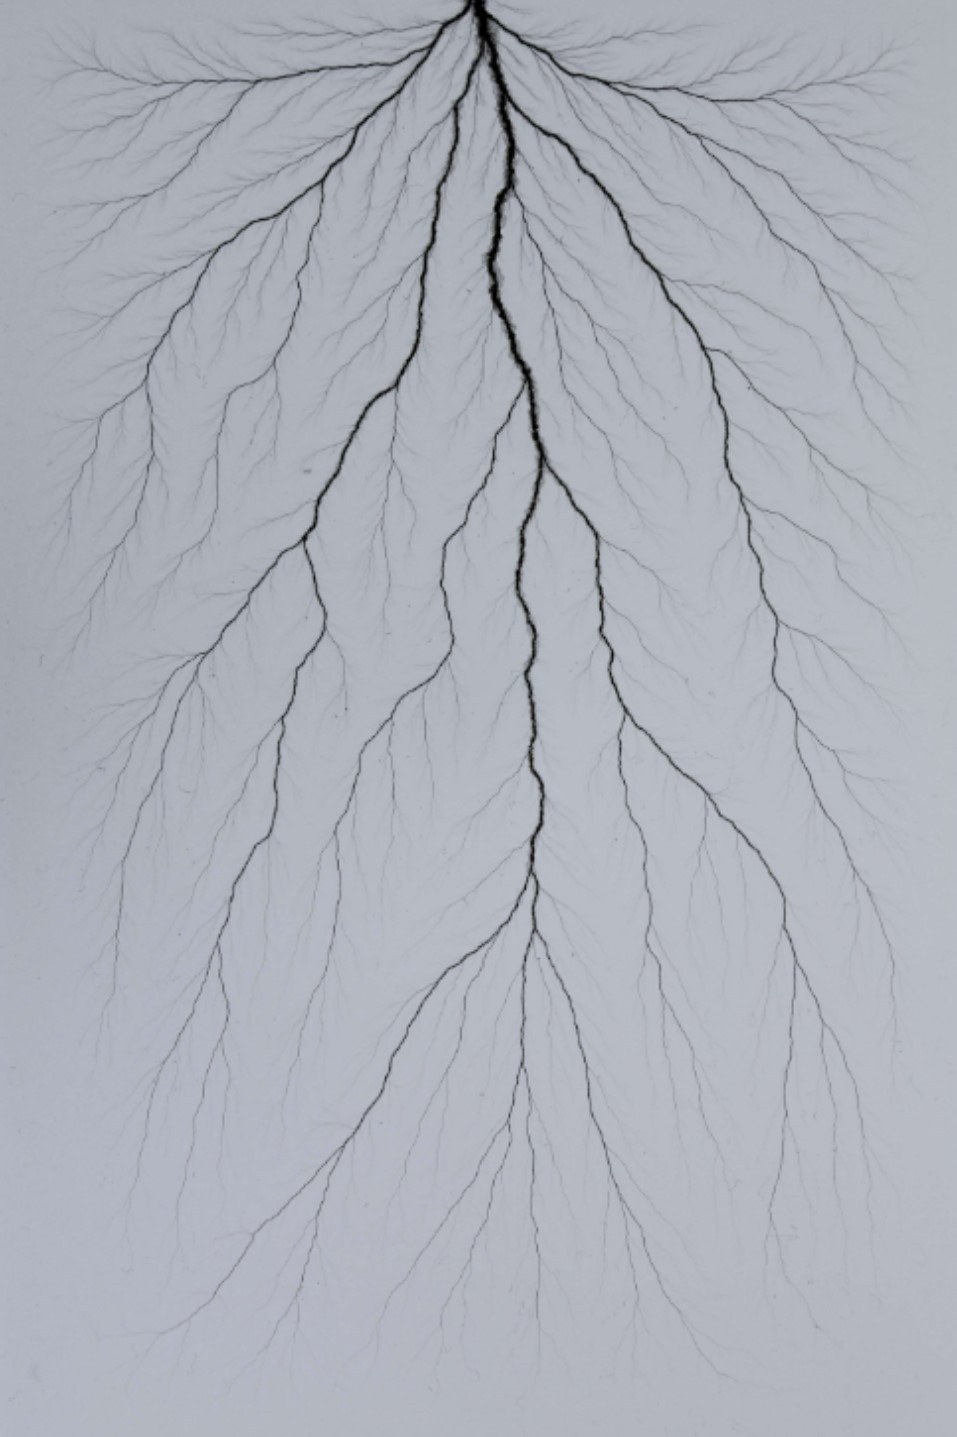
\includegraphics[height=0.19\textheight]{figs/lichtenberg_figure.jpg}}
      \quad
      \subfloat[]{\label{chicken}
      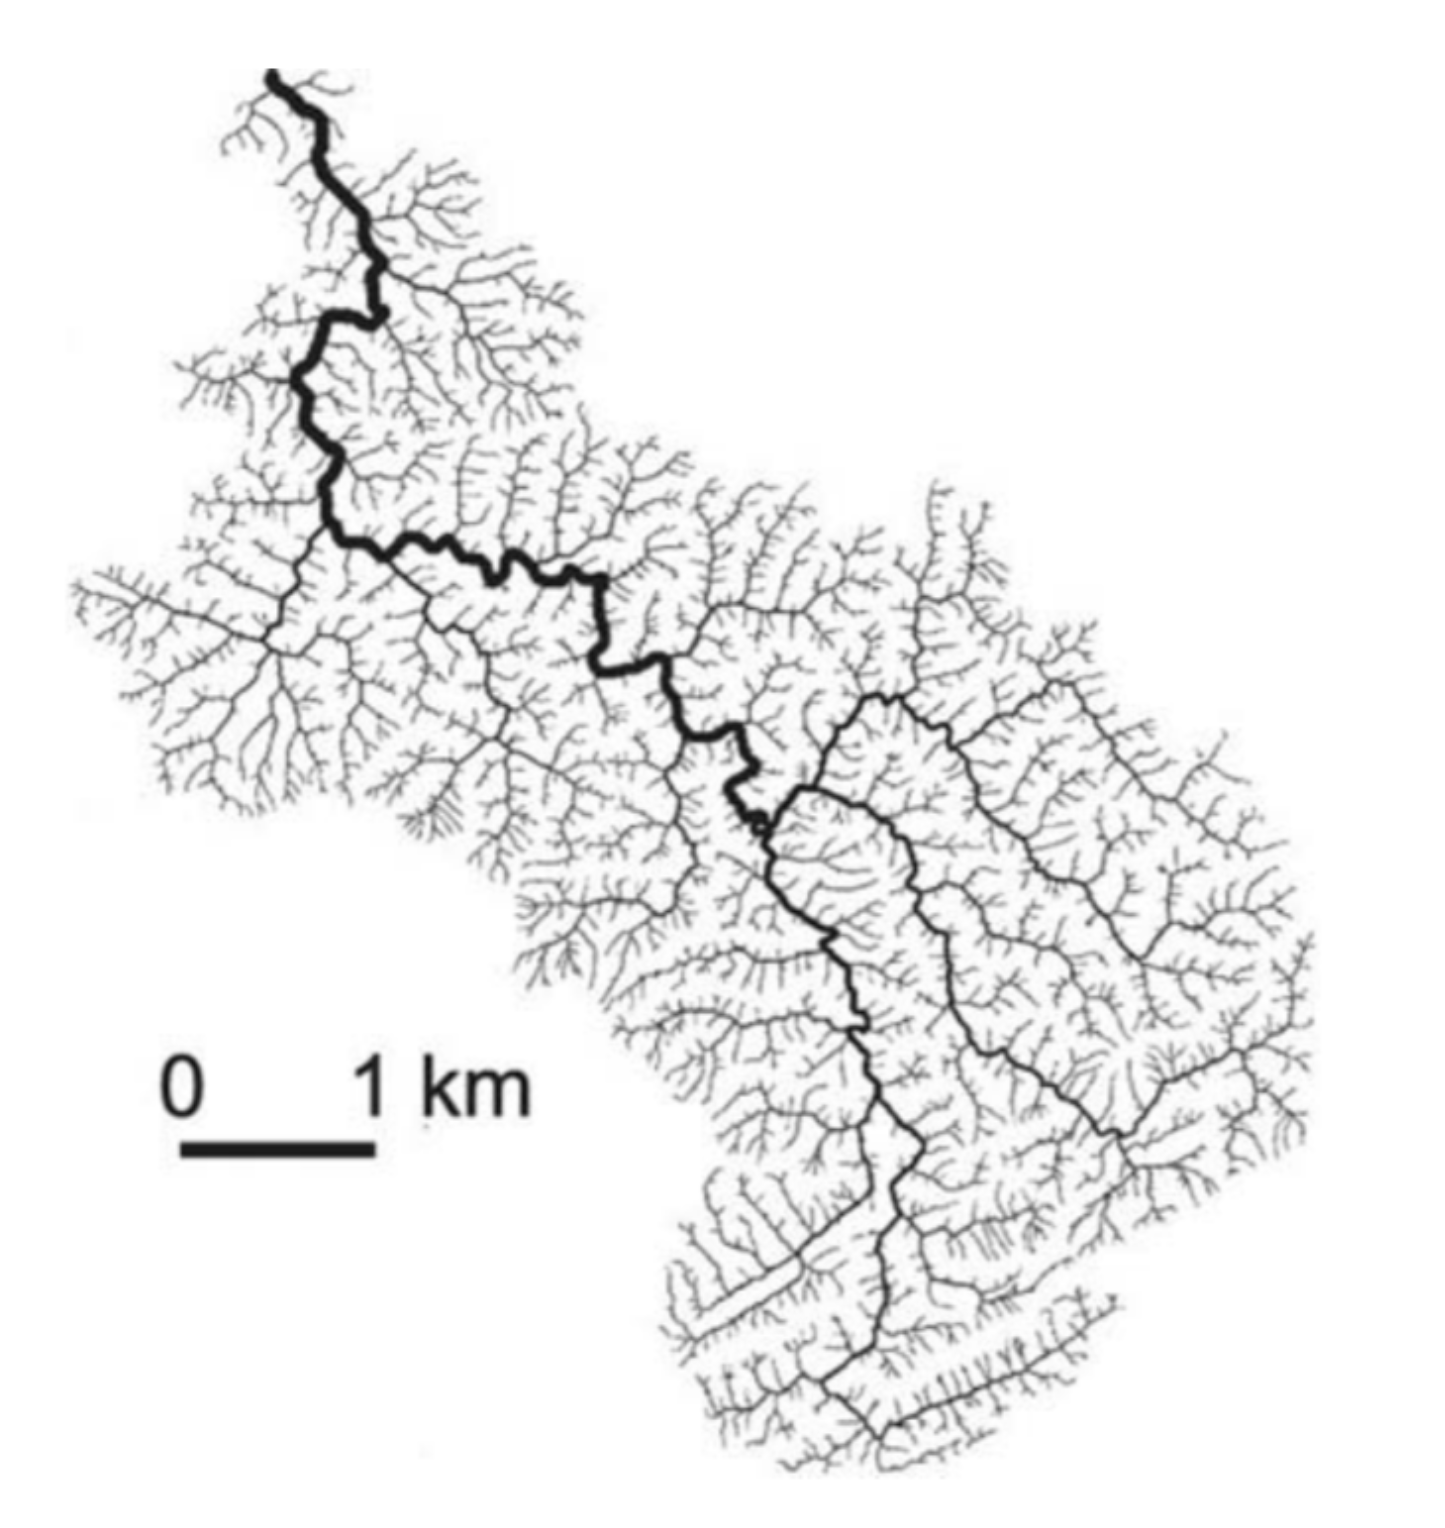
\includegraphics[height=0.19\textheight]{figs/dry_tug_fork_california.png}}
      \quad
      %\hspace{-10pt}
      \subfloat[]{\label{leaf}
      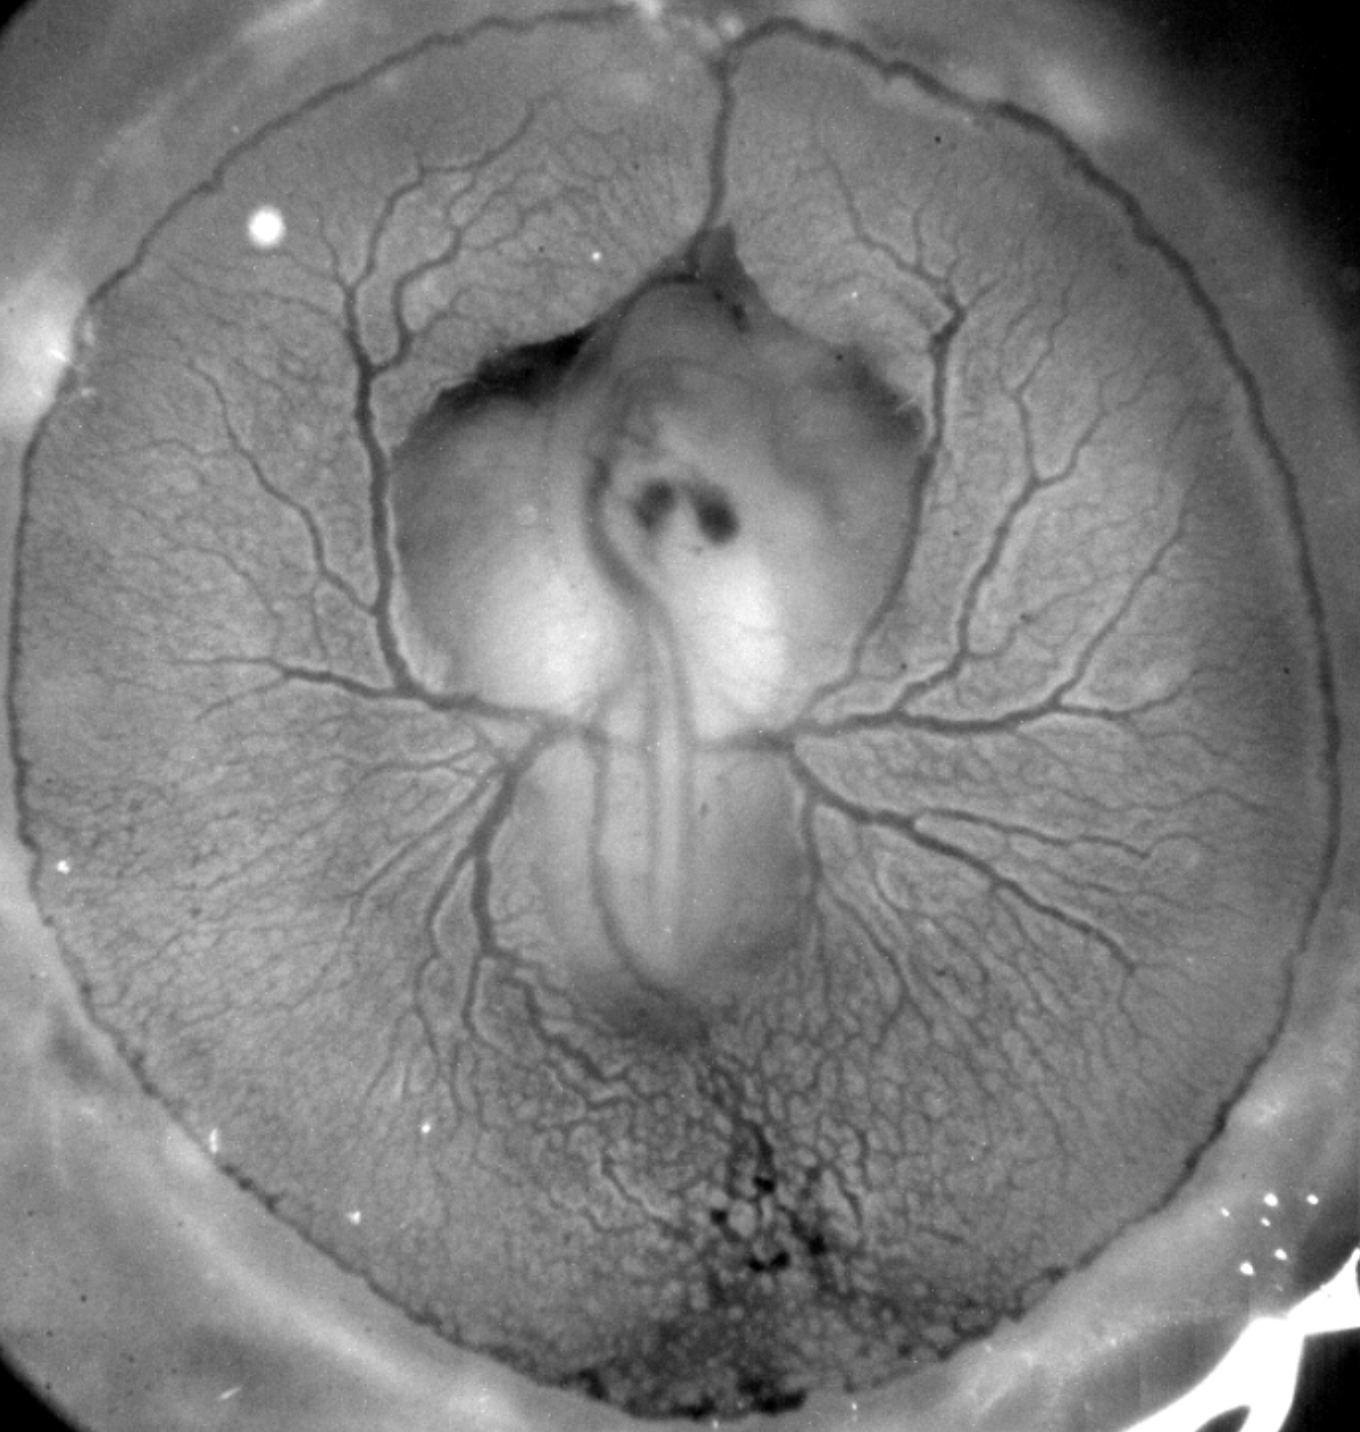
\includegraphics[height=0.19\textheight]{figs/chicken_yolk_sac.png}}
      \caption{Przykłady rozgałęzionych sieci przestrzennych w przyrodzie: (a)~Figura Lichtenberga \cite{paulslab} (b)~Dorzecze Dry Tug Fork w Kalifornii \cite{ball2009branches} (c)~Naczynia krwionośne na worku żółtkowym \cite{Clement2017tissue} (podziękowania dla Annemiek JM Cornelissen)}
      \label{networks_in_nature}
    \end{figure}
 
      Istotną cechą rozwoju sieci jest ścisłe sprzężenie pomiędzy geometrią a dynamiką. Środowisko napędzające wzrost i sieć współewoluują w czasie, w miarę ewolucji sieć zmienia warunki brzegowe dla pola. Rozwój sieci w odpowiedzi na otaczające pole składa się z dwóch głównych procesów: (i) rozszerzenie gałęzi oraz (ii) rozwidlenie końcówki na dwie (lub więcej) gałęzie. Aby zrozumieć koewolucja sieci i pola, ważne jest  zrozumieć w jaki sposób wzrost i procesy bifurkacyjne są powiązane z charakterystyką pól napędowych, takich jak na przykład gradient pola w okolicy czubka. Gdy poznamy \textit{zasady wzrostu}, możemy przewidzieć ewolucję geometrii sieci na podstawie jej wcześniejszej konfiguracji. \par
      
      Taką procedurę zastosowano do sieci rzecznych \cite{devauchelle2012ramification, petroff2013bifurcation, cohen2015path, yi2017symmetric, devauchelle2017laplacian}, lepkich palców \cite{pecelerowicz2016stabilizing} lub wzrost koralowców \cite{kaandorp2001algorithmic_Chapter4.4}, co prowadzi do jakościowo i ilościowo zbliżonych geometrii sieci do tych obserwowanych w przyrodzie. Jednak w wielu praktycznych przypadkach szczegóły reguł wzrostu są: nieznany, a czasową ewolucję wzorca można zaobserwować tylko w jednym przypadku czasu, ponieważ dynamika wzrostu może być po prostu zbyt wolna, jak np. w przypadku rzeki sieci, w których końcówki kanałów mogą poruszać się z prędkością mniejszą niż kilka milimetrów rocznie. Rodzi to następujące pytanie: czy możemy wydedukować regułę wzrostu z chwilowego 1 migawka konfiguracji sieci i opis ewolucji otaczającego środowiska w odpowiedzi na geometrię sieci? Rzeczywiście, geometria sieci ukrywa informacje o jego przeszłej konfiguracji, która jest nieodłącznie związana z dynamiką wzrostu.

      TODO: tutaj trzeba opisać mój przypadek.


  \chapter{Model teoretyczny}

    Aby zilustrować powyższe koncepcje, skupiamy się teraz na konkretnej sieci, a mianowicie sieci rzecznej. Ogólnie rzecz biorąc, jest to przykład wzrostu w odpowiedzi na pole dyfuzyjne. Tutaj pole jest połączone z siecią poprzez warunki brzegowe. Wiele innych naturalnych procesów wzrostu może być opisanych przez taki system, jak na przykład tworzenie się naczyń krwionośnych \cite{nguyen2006dynamics}, wzorce rozpuszczania w ośrodkach porowatych \cite{szymczak2011initial}, wyładowanie elektryczne \cite{niemeyer1984fractal} ta inne. W przypadku sieci rzecznych to pole dyfuzyjne opisuje wysokość zwierciadła wód gruntowych.

    Mówiąc o sieciach rzecznych, woda może dostać się do rzeki na dwa różne sposoby: (i) przez spływ powierzchniowy lub (ii) przez zbiornik wód podziemnych. W pierwszym przypadku woda (najczęściej z opadów atmosferycznych) nie zapada się pod ziemię i spływa po powierzchni bezpośrednio do koryta rzeki (jasnoniebieskie strzałki na rys.~\ref{pow_wsiakanie}). Taki scenariusz można zaobserwować w rejonach, gdzie grunt jest nieprzepuszczalny, a opady są tak intensywne, że woda nie zdąży zatopić się w ziemi.

    \begin{figure}[H]
      \centering
      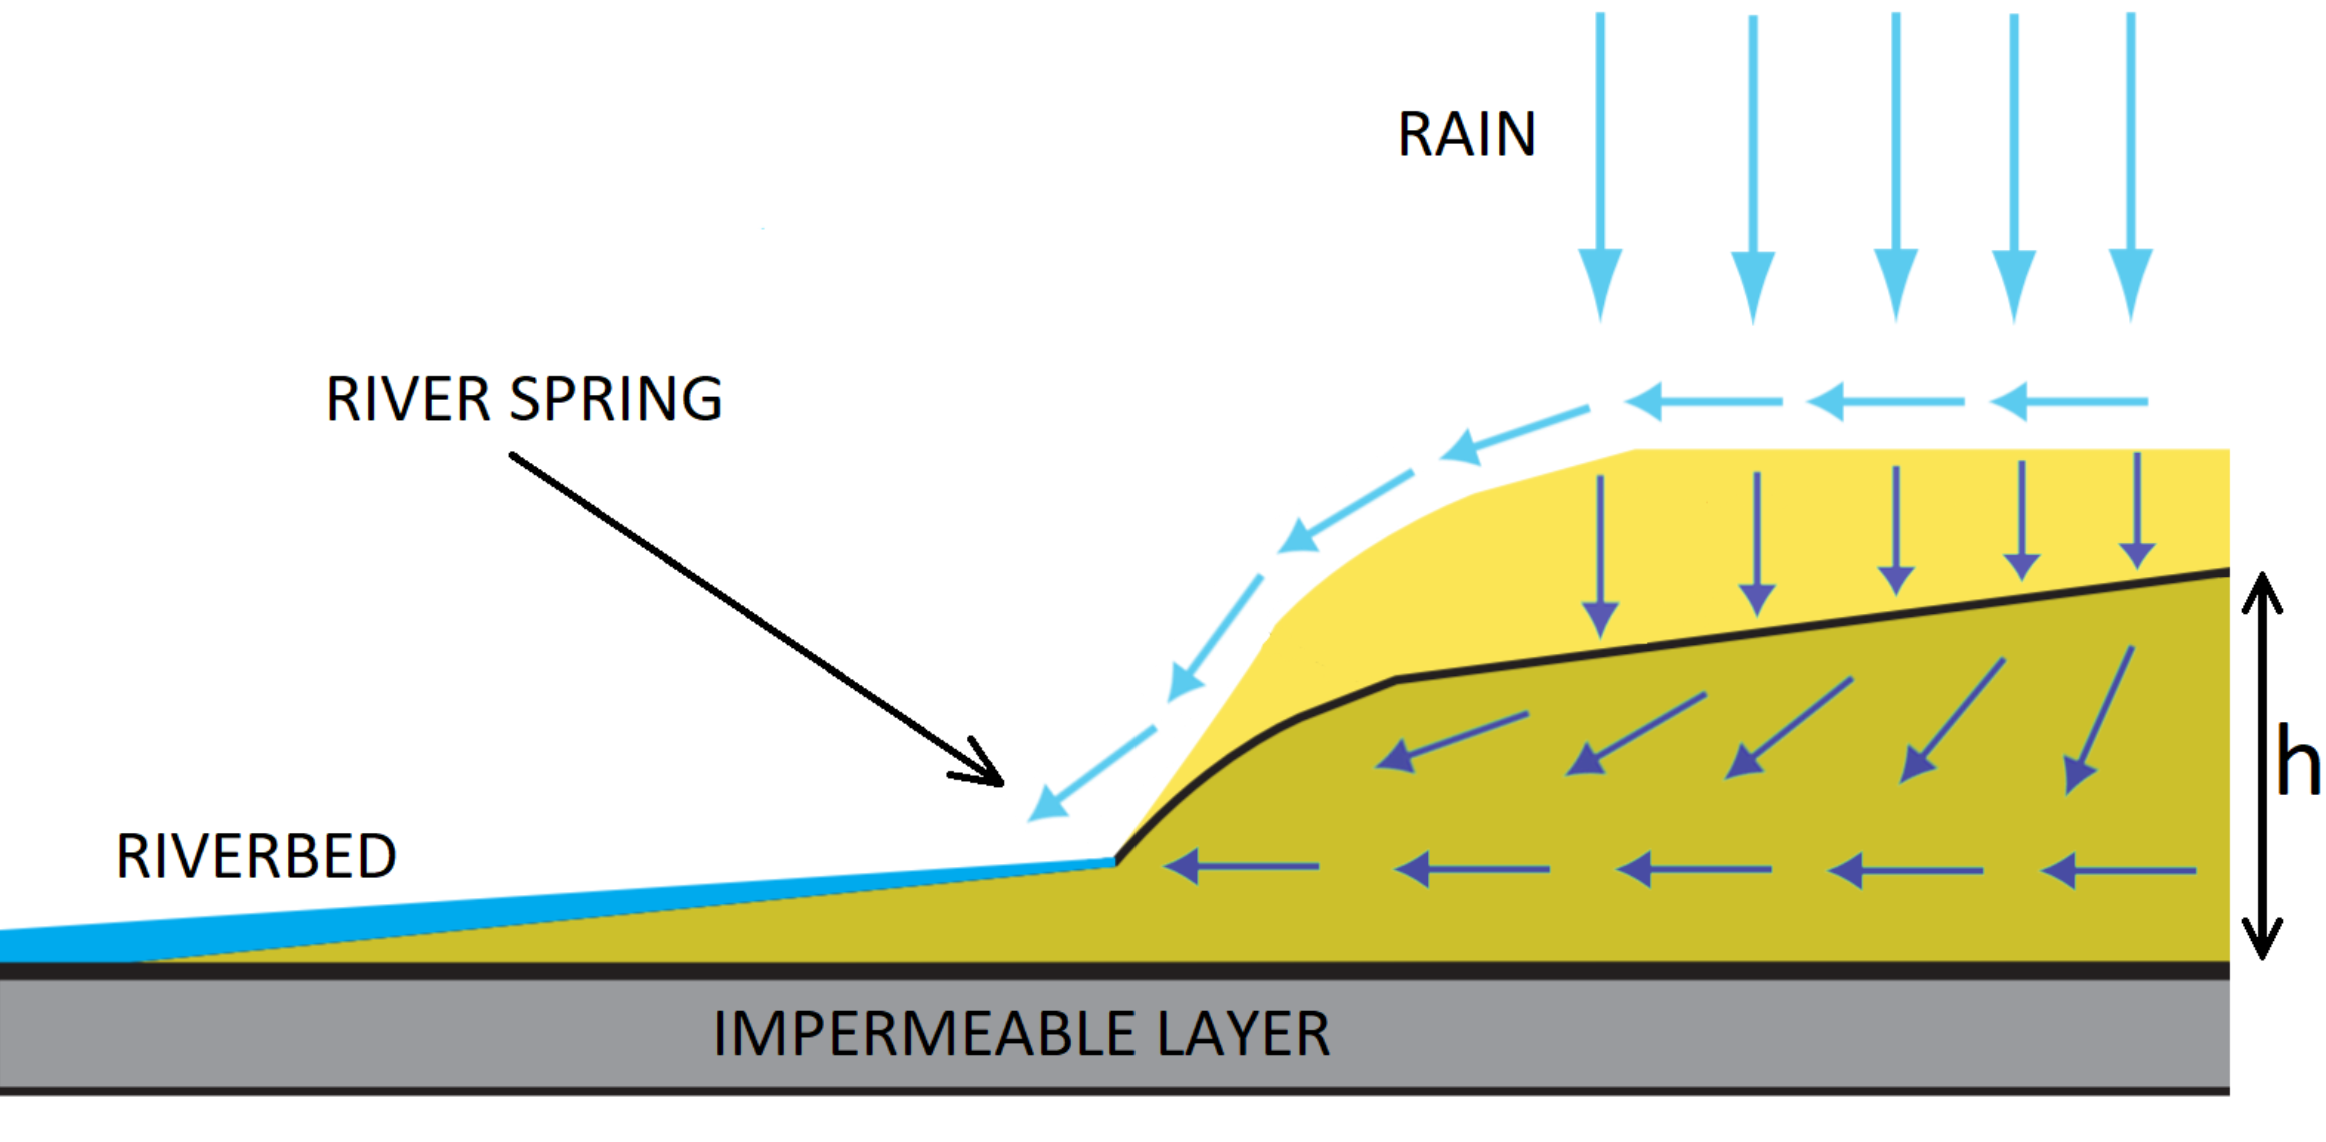
\includegraphics[width=1\textwidth]{figs/pow_wsiakanie_eng.png}
      \caption { Cross section of a river valley after Ref. \cite{berhanu2012shape}. Light blue arrows indicate surface runoff, whereas dark blue show water sinking into the ground. Yellow area is permeable ground, where dark yellow represent groundwater reservoir (black line marks groundwater table, which height is $h$). Riverbed lays directly on impermeable layer.}
      \label{pow_wsiakanie}
    \end{figure}

    Jednak zawsze, gdy grunt jest wystarczająco przepuszczalny, woda może zatopić się w ziemi zamiast spływać w dół (ciemnoniebieskie strzałki na rys.~\ref{pow_wsiakanie}). Woda najpierw gromadzi się w zbiorniku wód podziemnych, a następnie pod wpływem ciśnienia hydrodynamicznego wypływa ze źródła rzeki. Proces ten powoduje erozję źródła, ponieważ woda przeciera materiał, z którego składa się ziemia wokół źródła (np. piasek).

    \begin{wrapfigure}{r}{0.5\textwidth}
      \begin{center}
        \vspace{-20pt}
        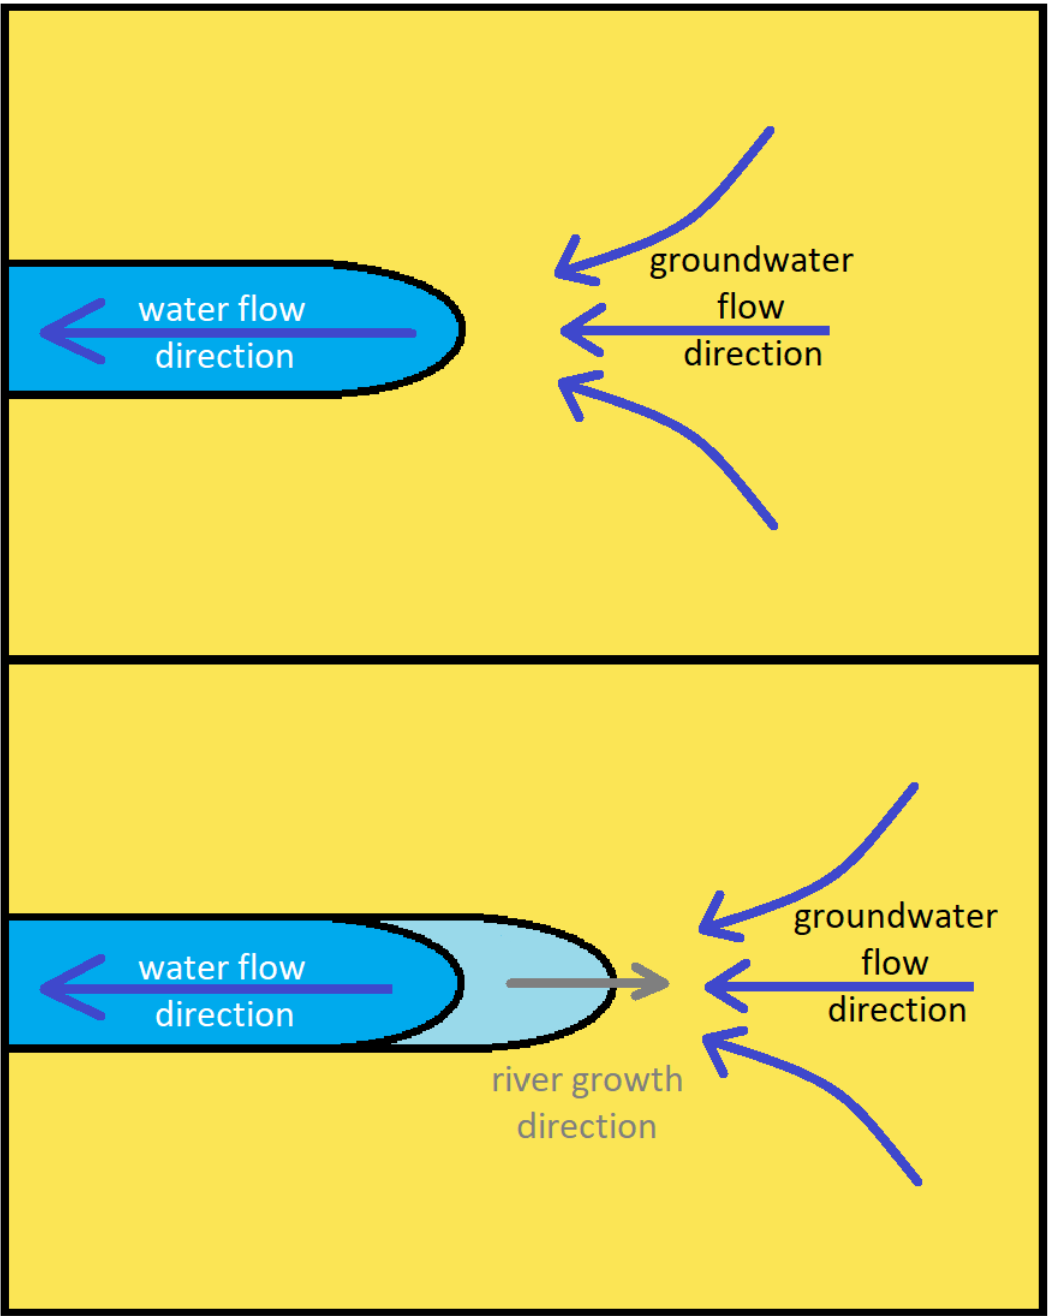
\includegraphics[width=0.45\textwidth]{figs/zrodlo_eng.png}
      \end{center}
      \vspace{-20pt}
      \caption{Top view on the growing river}
      \vspace{0pt}
      \label{zrodlo}
    \end{wrapfigure}

    Stąd, wbrew intuicji, rzeki nie rosną w kierunku przepływu wody. Erozja w okolicy źródła powoduje jej względny ruch w kierunku przeciwnym do przepływu wody (rys.~\ref{zrodlo}). Ta erozja wsteczna jest odpowiedzialna za rozszerzanie się i rozdzielanie rzek (tzw. bifurkacja) oraz ogólną ewolucję sieci rzecznych.

    Chociaż zaniedbanie spływu powierzchniowego nie może wyjaśnić ewolucji sieci rzecznej na obszarach suchych lub w górach, wiele sieci rzecznych wydaje się być zasilanych głównie przez przepływ wód gruntowych (zob. Ref.~\cite{schumm1995ground, petroff2011geometry, seybold2017climate} i rozdział~\ref{chapter:validation}). Pierwszy ilościowy model opisujący ewolucję takich rzek przedstawił w 1980 r. Dunne \cite{dunne1980formation}. Bardziej szczegółowe modele zaproponowano na przykład w grupie Daniela Rothmana z MIT (Refs.~\cite{petroff2012four, devauchelle2012ramification}), gdzie autorzy powiązali wysokość zwierciadła wód gruntowych z kierunkiem i prędkością wzrostu rzeki.

    Oprócz wspomnianego wcześniej zaniedbania spływu powierzchniowego, model grupowy Rothmana pomijał zmienną wysokość nieprzepuszczalnej warstwy, na której leży rzeka, co miałoby wpływ na kształt zwierciadła wód gruntowych. Zakładają również, że przepuszczalność powierzchni jest stała. Model uwzględnia jedynie rozwój sieci poprzez ruch źródeł. W rzeczywistości woda płynąca w rzece nieustannie ma wpływ na brzeg rzeki i jej ukształtowanie -- pojawiają się meandry, koryto rozszerza się. Dodatkowo sama rzeka traktowana jest jako obiekt liniowy o zerowej szerokości. Nie jest to dalekie od rzeczywistości, ponieważ szerokość pojedynczego koryta jest znikoma w skali całej sieci rzecznej.

    \section{Wody podziemne}

      Aby określić ilościowo erozję w okolicy źródła, musimy opisać dynamikę wody po opadnięciu w grunt. W dalszych rozważaniach skupimy się na dynamice wody w warstwie wodonośnej, zaznaczonej na rys.~\ref{pow_wsiakanie} kolorem ciemnożółtym.

      Wodę zgromadzoną w zbiorniku wód podziemnych opisuje prawo Darcy'ego \cite{darcy1856fontaines}:
      
      \begin{equation}
        \vec{u}=-\frac{\kappa}{\mu} \nabla p
      \end{equation}	
      
      Równanie to opisuje prędkość filtracji ($\vec{u}$) płynu o lepkości dynamicznej $\mu$ przez ośrodek porowaty (np. piasek lub skały) o przepuszczalności $\kappa$ pod ciśnieniem $p$. Zauważ, że rzeczywista prędkość płynu ($u_a$) jest lokalnie wyższa: $u_a = u / n_e$, gdzie $n_e$ to porowatość. Ponieważ płyn może przepływać tylko przez pory i musi omijać materiał w medium (np. ziarna piasku), strumień masy w danym punkcie przepływający przez medium jest opisany przez prędkość filtracji.
    
      Aby obliczyć, ile wody przepływa przez określony punkt na płaszczyźnie $xy$, gdzie sieć się rozrasta, po prostu całkujemy prędkość Darcy'ego w danych współrzędnych $xy$ wzdłuż osi poziomej $z$ (wysokość zbiornika):
      
      \begin{equation}
        \vec{q}(x,y)=\int \vec{u}(x,y,z)\textrm{d}z
      \end{equation}
    
      Teraz korzystamy z założenia Dupuit \cite{dupuit1863etudes}, które mówi, że wody gruntowe płyną poziomo. Ponadto zakładamy, że ciśnienie powodujące przepływ jest po prostu ciśnieniem hydrostatycznym $p = \rho g h $ ($\rho$ -- gęstość wody, $g$ -- przyspieszenie grawitacyjne, $h$ -- wysokość Tabela wód podziemnych). Dla takiego ciśnienia $\nabla p$ jest niezależne od współrzędnej $z$, a powyższa całka upraszcza się do iloczynu prędkości filtracji $\vec{u}$ i wysokości słupa wody $h(x, y)$ w danym miejscu:
      
      \begin{equation}
        \label{qq}
        \vec{q}(x,y)=h\vec{u}=-h \frac{\kappa}{\mu} \nabla(\rho g h)=-\nabla \left(\frac{\kappa \rho g}{2\mu}h^2(x,y)\right) = - \nabla \phi(x,y) \,,
      \end{equation}
      
      gdzie wprowadziliśmy potencjał $\phi(x,y)$:
      
      \begin{equation}
        \phi(x,y) = \frac{\kappa \rho g}{2\mu}h^2(x,y) \,.
      \end{equation}

      Zauważ, że w równaniu \eqref{qq} wszystkie operatory różniczkowe działają w płaszczyźnie $xy$.
    
      Na koniec wyprowadzamy równania opisujące pole $\phi$ z równania ciągłości, uwzględniając opady (opisane przez średnią objętość opadów na jednostkę czasu i powierzchnię — $P$). Zmianę masy kolumny płynu ($M$) zamkniętej w obszarze $S$ (widok z góry na Rys. \ref{zachowanie_masy}) można opisać następująco:
    
      \begin{wrapfigure}{r}{0.25\textwidth}
        \vspace{-8pt}
        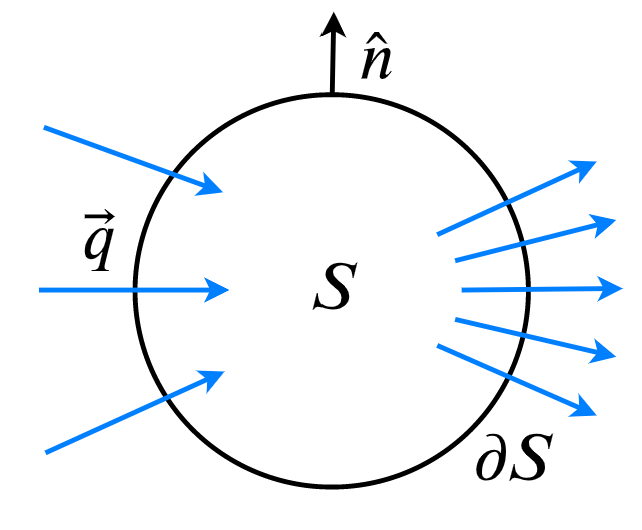
\includegraphics[width=0.25\textwidth]{figs/zachowanie_masy.png}
        \vspace{-15pt}
        \caption{}
        \vspace{-1000pt}
        \label{zachowanie_masy}
      \end{wrapfigure}

      \begin{gather*}
        \frac{\partial M}{\partial t}=- \int\limits_{\partial S} \vec{q}\cdot \hat{n} \ \textrm{d}l + \int\limits_S P \ \textrm{d}S
        \\
        \frac{\partial}{\partial t} \int\limits_S \rho h \ \textrm{d}S=\int\limits_S \left(-\nabla \cdot \vec{q} + P\right)\textrm{d}S
        \\
        \rho \frac{\partial h}{\partial t}=-\nabla \cdot \vec{q} + P
      \end{gather*}	

      W tym miejscu należy skomentować skale czasowe w rzeczywistych systemach. Średni czas między opadami to 10 dni, a średni czas przepływu wody przez system to $10^4$ dni. Oznacza to, że wahania wysokości zwierciadła wód gruntowych $h$ są bardzo małe i jako $P$ możemy przyjąć średnią roczną wielkość opadów. Ponadto szybkość wzrostu sieci rzecznej szacuje się na około 1~mm/rok, a charakterystyczny czas zmian geometrii to $10^4$ lat. To z kolei oznacza, że w skalach czasowych odpowiadających wzrostowi sieci rzecznej możemy pominąć $ \frac{\partial h} {\partial t} $ w równaniu ciągłości, otrzymując:
      
      \begin{equation}
    		\nabla \cdot \vec{q} = P \,.
    	\end{equation}
      
      Używając wcześniej zdefiniowanego potencjału $\phi$ otrzymujemy równanie Poissona:
      
      \begin{equation}
        \label{poisson}
    		\Delta \phi = -P/\kappa
    	\end{equation}
      
      lub równanie Laplace'a, gdzie nie ma opadów ($P=0$):
      
      \begin{equation}
        \label{laplace}
    		\Delta \phi = 0 \,.
    	\end{equation}	

      Równania te muszą być uzupełnione odpowiednimi warunkami brzegowymi. W naszym przypadku zakładamy, że rzeka płynie bezpośrednio po warstwie nieprzepuszczalnej (przy $h = 0$), czyli $\phi = 0$ na całej jej długości. Dodatkowo granice domeny są często nieprzepuszczalne, co można zapisać jako odblaskowy warunek brzegowy ($\frac{\partial \phi} {\partial \vec{n}} = 0$). Wreszcie, gdy nie ma opadów, zakładamy, że woda wchodzi do układu przez jedną z granic (na przykład z odległych lodowców) -- można to opisać jako stały przepływ pola $\phi$ wzdłuż rozważanej ściany ($\ frac{\partial \phi} {\partial \vec{n}} = const.$).
      
      W ten sposób udało nam się zredukować trójwymiarowy problem przepływu płynów do obliczenia dwuwymiarowego potencjału, który niesie pełną informację o dynamice wód gruntowych. W kolejnej części pokażemy, jak sama geometria rzek może zostać zredukowana do jednowymiarowych palców.

    \section{Przybliżenie rzeki cienkim palcem}

      Aby wyjaśnić przejście od dwuwymiarowych rzek do jednowymiarowych obiektów je reprezentujących, tak zwanych cienkich palców, posłużymy się innym przykładem procesu wzrostu w odpowiedzi na pole Laplace'a -- lepkim palcowaniem. Ten podstawowy, hydrodynamiczny przykład wzrostu Laplace'a został sformułowany przez Muskata w 1937 r. \cite{muskat1937flow} i opisuje ewolucję granicy faz między dwiema fazami -- na przykład dwoma płynami, gdzie jedna najeżdża i wypycha drugą. W tym konkretnym przypadku pole $\phi$ to ciśnienie, a $\kappa$ to współczynnik ruchliwości. Pomijając ruchliwości fazy inwazyjnej prowadzi do uproszczonej jednofazowej wersji tego problemu z warunkiem brzegowym Dirichleta na rosnącej powierzchni międzyfazowej. Zatem front ruchomy jest izolinią pola ciśnienia ($\phi = 0$). Front rośnie wzdłuż linii pola z prędkością ($\vec{v}$) proporcjonalną do gradientu pola ciśnienia:
      
      \begin{equation}
        \vec{v} \propto \nabla \phi
      \end{equation}

      W niektórych przypadkach front inwazyjny staje się niestabilny, co prowadzi do powstania tzw. palców. Niestabilności pojawiające się w takim układzie zostały przeanalizowane przez Hilla w 1952 roku w swojej pracy na temat wypierania cieczy cukrowej przez wodę w procesie rafinacji cukru \cite{hill1952channeling}. Jednak prawdziwe zainteresowanie zjawiskiem lepkiego palcowania pojawiło się w 1958 r. wraz z przełomowym artykułem Saffmana i Taylora \cite{saffman1958penetration}, w którym systematycznie badali pojawianie się wzorców w komórkach Hele-Shaw. Badana przez nich niestabilność stała się później znana jako niestabilność Saffmana-Taylora.

      Istnieje wiele zastosowań tego czysto hydrodynamicznego zjawiska i stojącej za nim matematyki w innych dziedzinach, takich jak tworzenie płuc \cite{clement2012branching,lubkin1995mechanism}, tworzenie jaskiń \cite{szymczak2011initial}, wzrost kolonii bakterii \cite{matsushita1990diffusion}, metaliczne dendryty rosną przez osadzanie elektrochemiczne \cite{brady1984fractal}, palcy spalania \cite{zik1999fingering}, przebudowę naczyń krwionośnych w woreczku żółtkowym podczas rozwoju zarodka kurczaka \cite{nguyen2006dynamics} lub naczynia krwionośne w nas \cite{schneider2012tissue}. Systemy te są zwykle opisywane jako ewolucja ciągłego interfejsu między dwiema fazami (rys. \ref{continuous_to_thin}) z pewnym mechanizmem regularyzacji na małą skalę, takim jak napięcie powierzchniowe. Bez tej regularyzacji strumień pola skoncentrowany na końcach faworyzuje bardzo cienkie palce i prowadzi do ich nieskończenie szybkiego wzrostu -- tak zwanej katastrofy ultrafioletowej \cite{shraiman1988singularities}.

      Istnieje jednak również inny sposób na uniknięcie katastrofy ultrafioletowej, który nie wiąże się z napięciem powierzchniowym. Dokładnie jak piorunochron chroniący budynki przyciąga pioruny, końcówki palców w sieciach skupiają strumień pola. Struktury podobne do sieci we wzroście Laplace'a pojawiają się w wyniku tej koncentracji strumienia. Największy gradient pola występuje na czubkach palców, co sprawia, że są one obszarami najintensywniejszego wzrostu, stąd palce z czasem ulegają stopniowemu wydłużeniu. Jeśli jednocześnie odległości między palcami są znacznie większe niż ich szerokość, można przybliżyć palce cienkimi liniami, rozciągającymi się tylko na długości \cite{peterson1998singular,carleson2002laplacian,gubiec2008fingered} (rys. \ref{continuous_to_thin}). To przybliżenie nazywa się modelem cienkiego palca -- zamiast śledzić ciągłą granicę, zakłada się, że wzrost ma miejsce tylko w dyskretnej liczbie punktów -- czubkach palców. Końcówki również mogą się rozgałęziać, dzieląc się na dwa palce potomne.

      \begin{figure}[h]
        \centering
        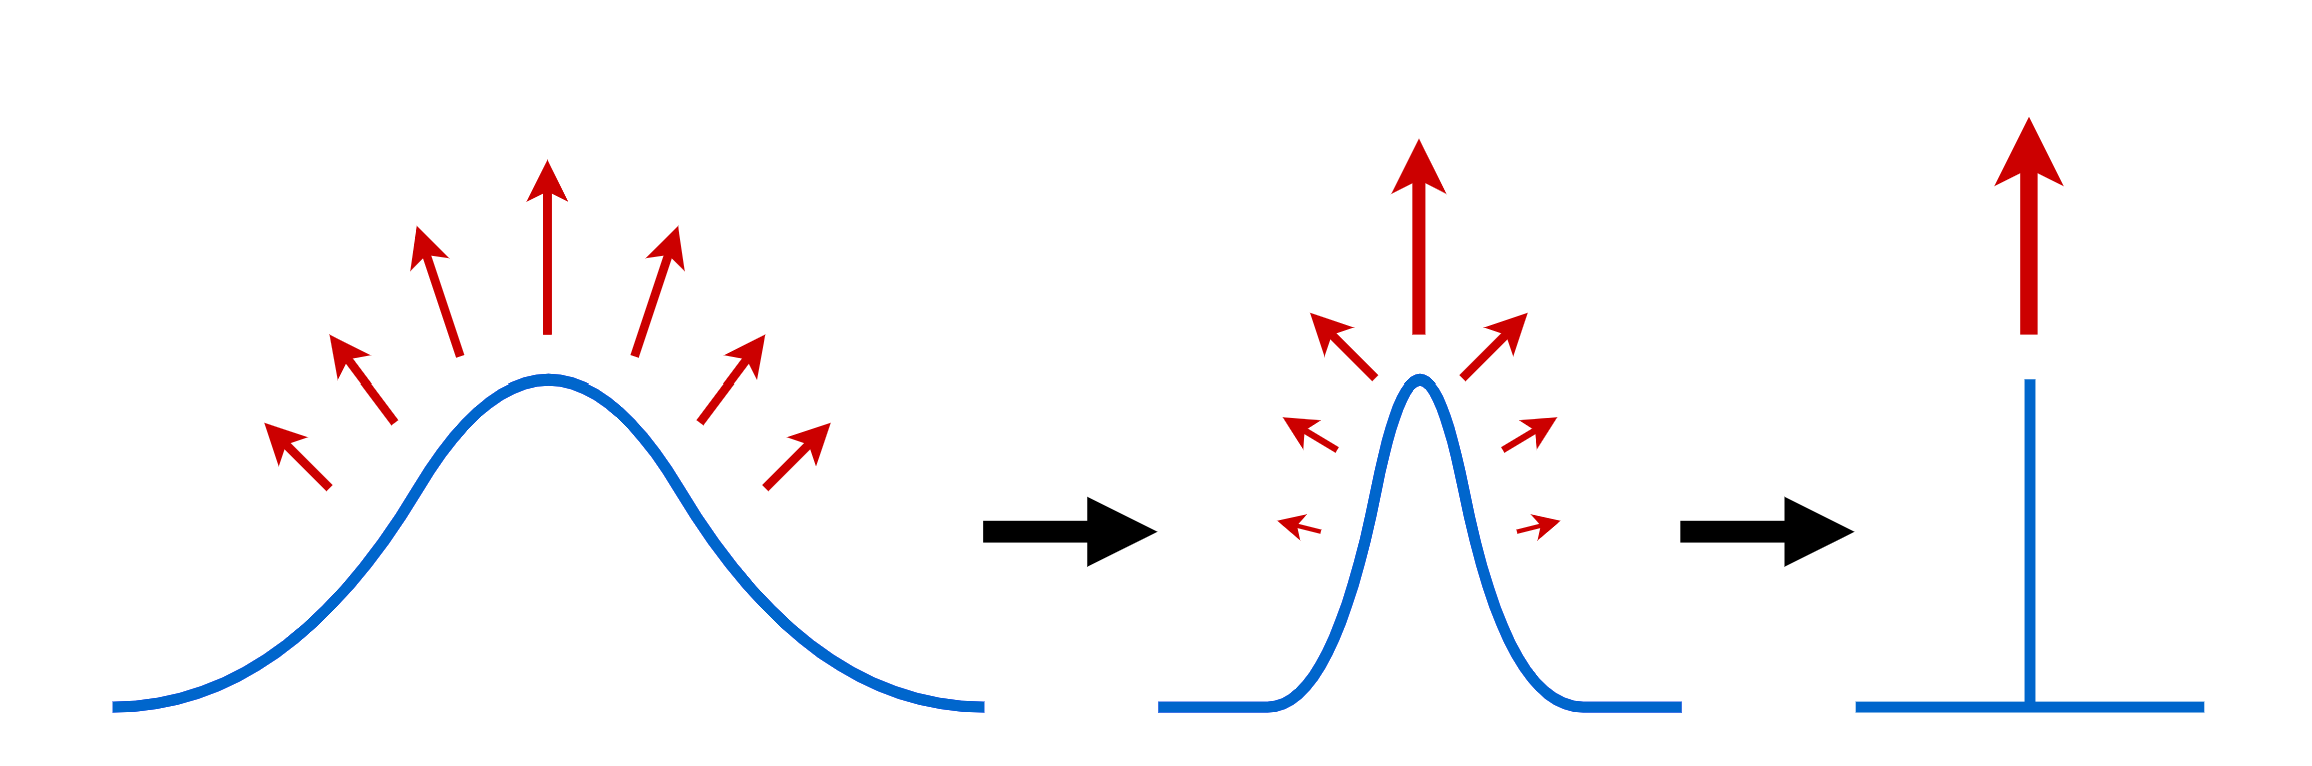
\includegraphics[width=0.9\textwidth]{figs/continuous_to_thin.png}
        \caption {Przejście od problemu ciągłego interfejsu do modelu cienkiego palca. Strzałki wskazują prędkość wzrostu interfejsu.}
        \label{continuous_to_thin}
      \end{figure}

      TODO: zdanie ponizej mozna wycofac imo.
      Problem ten można przeanalizować np. za pomocą map konforemnych \cite{loewner1923untersuchungen, gubiec2008fingered}. Posłużymy się tutaj metodą rozwiązania równania Laplace'a poprzez rozwinięcie rozwiązania na szereg Taylora na płaszczyźnie zespolonej \cite{petroff2013bifurcation}, co pozwoli nam wykorzystać metody numeryczne do analizy problemu.


    \section{Obserwacje i walidacja modelu}\label{chapter:validation}

      W pierwszej kolejności uzasadnijmy podejście wyjaśniające ewolucję sieci rzecznych erozją przesiąkającą związaną z odpływem wód gruntowych w źródłach. W 1980 r. motywacją Dunne do poszukiwania nowego opisu rozwoju sieci rzecznej była obserwacja obszaru w Vermont. Na granicy tego obszaru przebiegała droga zatrzymująca lądowy spływ wód, co uniemożliwiłoby rozwój sieci rzecznej pod drogą, gdyby rzeka była zasilana spływem powierzchniowym. Powstała tam jednak sieć rzeczna -- droga leżąca na powierzchni nie blokowała przepływu wód gruntowych \cite{dunne1980formation}. Pięć lat później, w 1985 roku, w Ref.~\cite{laity1985sapping} wykazano, że rzeki na płaskowyżu Kolorado są również zasilane przez wody gruntowe. Ponadto Lobkovsky \cite{lobkovsky2004threshold} wykazał, że spływ powierzchniowy przyczynia się do erozji tylko przy odpowiednio dużym nachyleniu terenu, co znacznie rozszerza zakres stosowalności modelu. Innym czynnikiem, który pozwala nam zaniedbywać spływ powierzchniowy, jest rodzaj gleby, w którą wcinają się rzeki. Przepuszczalny piasek lub porowate skały, takie jak piaskowiec, pozwalają wodzie opadać pod ziemię i gromadzić się w warstwie wodonośnej.

      Następnie, aby zweryfikować podejście oparte na modelu cienkich palców, Seybold et al. w Ref.~\cite{seybold2017climate, seybold2018branching} wykonali analizę statystyczną rzek rosnących na obszarach o różnej wilgotności i wykazali związek między klimatem a średnim kątem rozwidlenia w sieci. Można analitycznie wykazać, że kąt rozwarcia bifurkacji w modelu cienkiego palca wynosi $72^\circ$ \cite{hastings2001growth, carleson2002laplacian, gubiec2008fingered, devauchelle2012ramification} i widzimy, że ten kąt odpowiada obszarom wilgotnym na Rys.~\ref{klimat_katy}. Można to wytłumaczyć tym, że woda zwykle spływa po suchej glebie (np. na pustyniach), podczas gdy w wilgotnych regionach może łatwiej zapadać się w ziemię.

      \begin{figure}[H]
        % \vspace{-15pt}
        \centering
        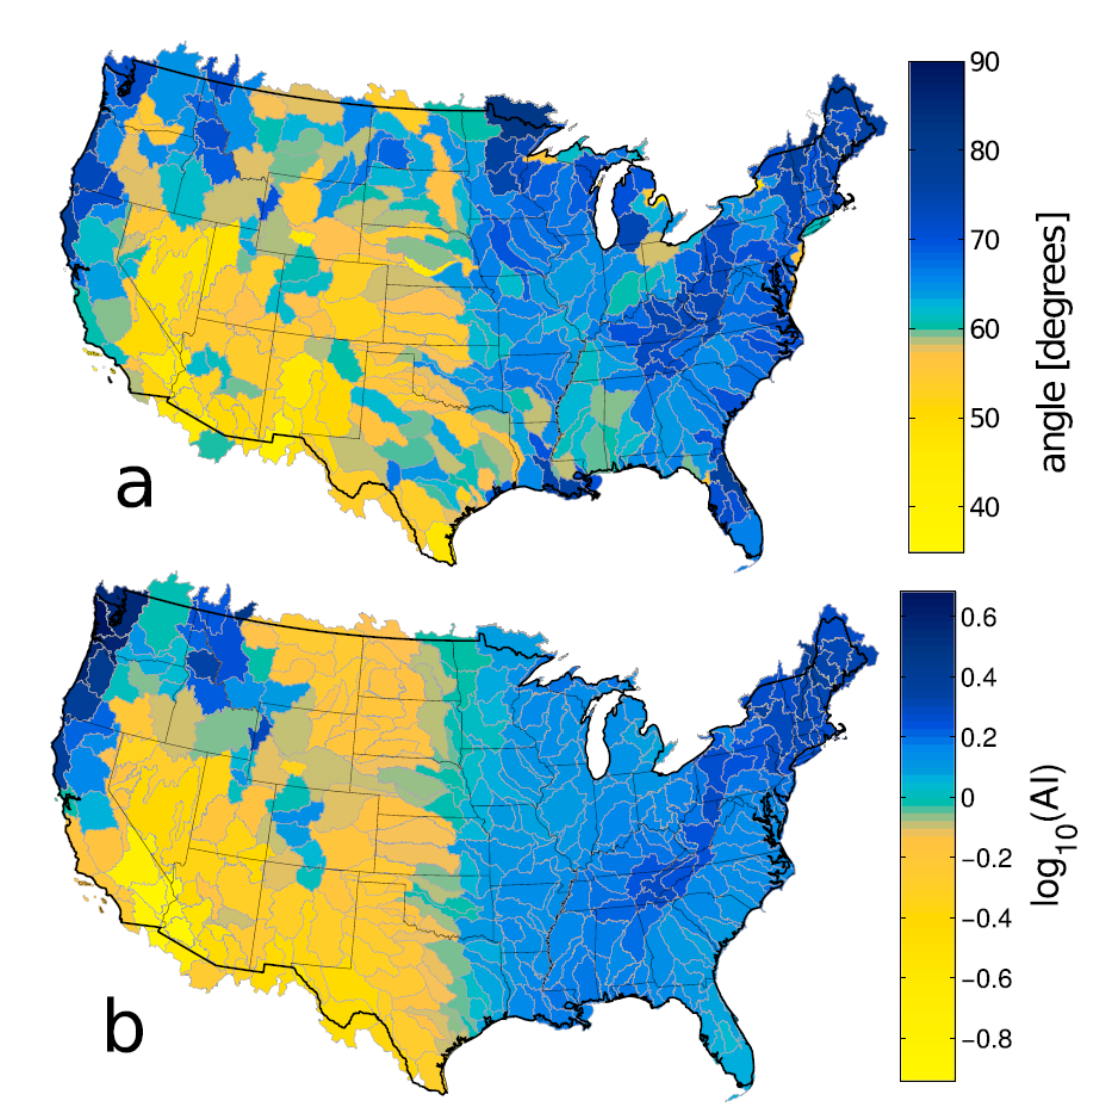
\includegraphics[width=0.45\textwidth]{figs/klimat_katy.png}
        % \vspace{-15pt}
        \caption{Porównanie średnich kątów rozgałęzień w sieciach rzecznych (a) z wilgotnością regionu (AI -- wskaźnik suchości) (b)}
        % \vspace{-5pt}
        \label{klimat_katy}
      \end{figure}

      Przykładami sieci rzecznych rozwijających się na polu Laplace'a są rzeki rosnące na wybrzeżu Nowej Zelandii \cite{schumm1986composite}. Zaopatrywane są w wodę z topniejących lodowców górskich, która następnie opada w ziemię i transportowana jest na duże odległości w zbiornikach wód podziemnych. Rys.~\ref{nowa_zelandia} pokazuje podobieństwo rzek w takim układzie do palców sięgających w kierunku odległego źródła wody TODO: remove this and add reference to stasiek work: uzyskanych w symulacjach.

      \begin{figure}[h]
        \centering
        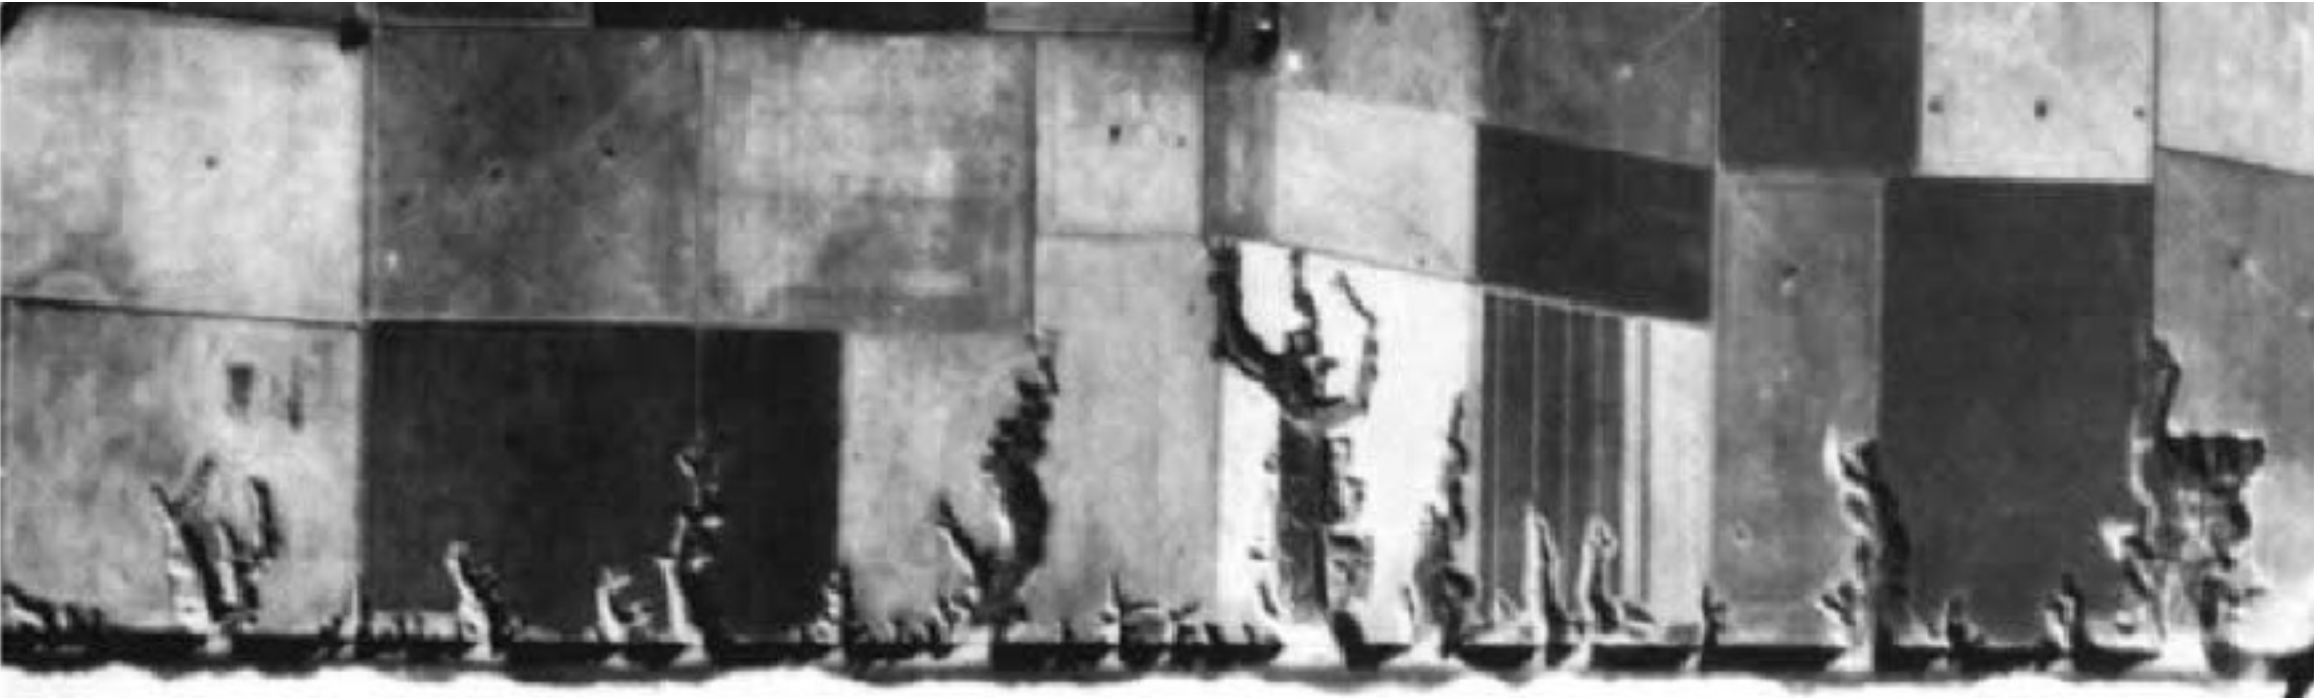
\includegraphics[width=1\textwidth]{figs/nowa_zelandia.png}
        \caption{Rzeki rosnące na polu Laplace'a na wybrzeżu Nowej Zelandii \cite{schumm1986composite}}
        \label{nowa_zelandia}
        \vspace{0pt}
      \end{figure}

      Większość rzek jest jednak zasilana przez lokalne opady. Przykładem tego typu sieci ewoluującej w polu Poissona jest sieć dopływów rzeki Apalachicola na Florydzie \cite{schumm1995ground}. Dla tej sieci rzecznej przeprowadzono szereg analiz w celu potwierdzenia stosowalności modelu wód podziemnych. W ref. \cite{petroff2013bifurcation} Petroff i in. zmierzyli kąty z 4966 bifurkacji i wykazali, że średni kąt $\alpha = 71,9^\circ \pm 0.8^\circ$, co jest bardzo zgodne z teoretyczną wartością $2\pi/5=72^\circ$ (rys. .~\ref{apalachicola_katy}). Dodatkowo rozwiązali numerycznie równanie Poissona dla fragmentu tej sieci, co przedstawiono na rys.~\ref{potencjal_floryda}a. Wykorzystując wyliczony potencjał uzyskali strumień wody na całym rozpatrywanym obszarze. Następnie zmierzono doświadczalnie strumień wody płynącej w rzekach, a porównanie teorii z eksperymentem przedstawiono na rys.~\ref{potencjal_floryda}b. Ponownie dane teoretyczne i eksperymentalne wykazują wysoki stopień zgodności.

      \begin{figure}[H]
        \centering
        \begin{minipage}{0.4\textwidth}
          \caption{Rozkład kątów bifurkacji oszacowany na podstawie 4966 cieków rozwidlonych w sieci rzecznej Apalachicola.}
          \label{apalachicola_katy}
        \end{minipage}
        \hspace{20pt}
        \begin{minipage}{0.5\textwidth}
          \centering
          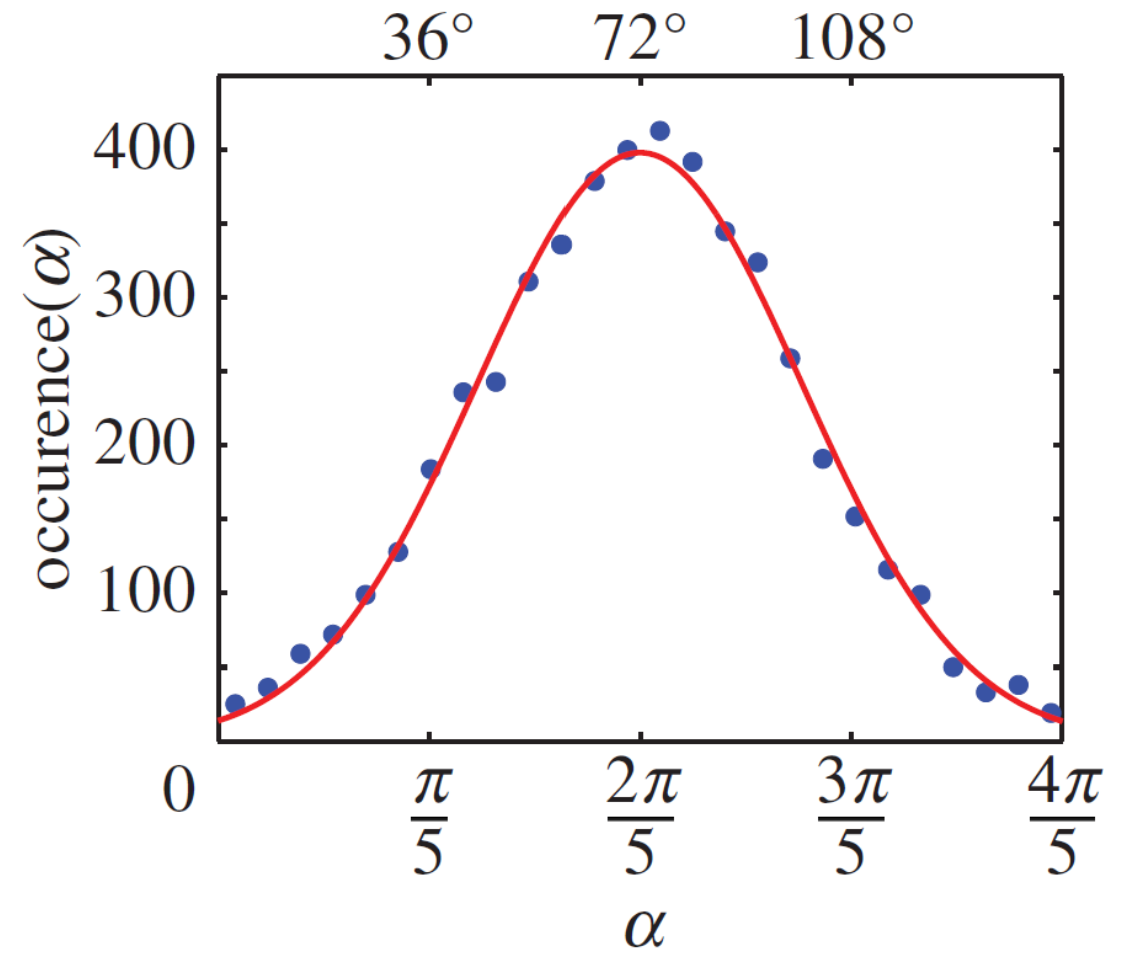
\includegraphics[width=1\textwidth]{figs/florida_angles.png}
          \end{minipage}
    \end{figure}  

    \begin{figure}[H]
      \centering
      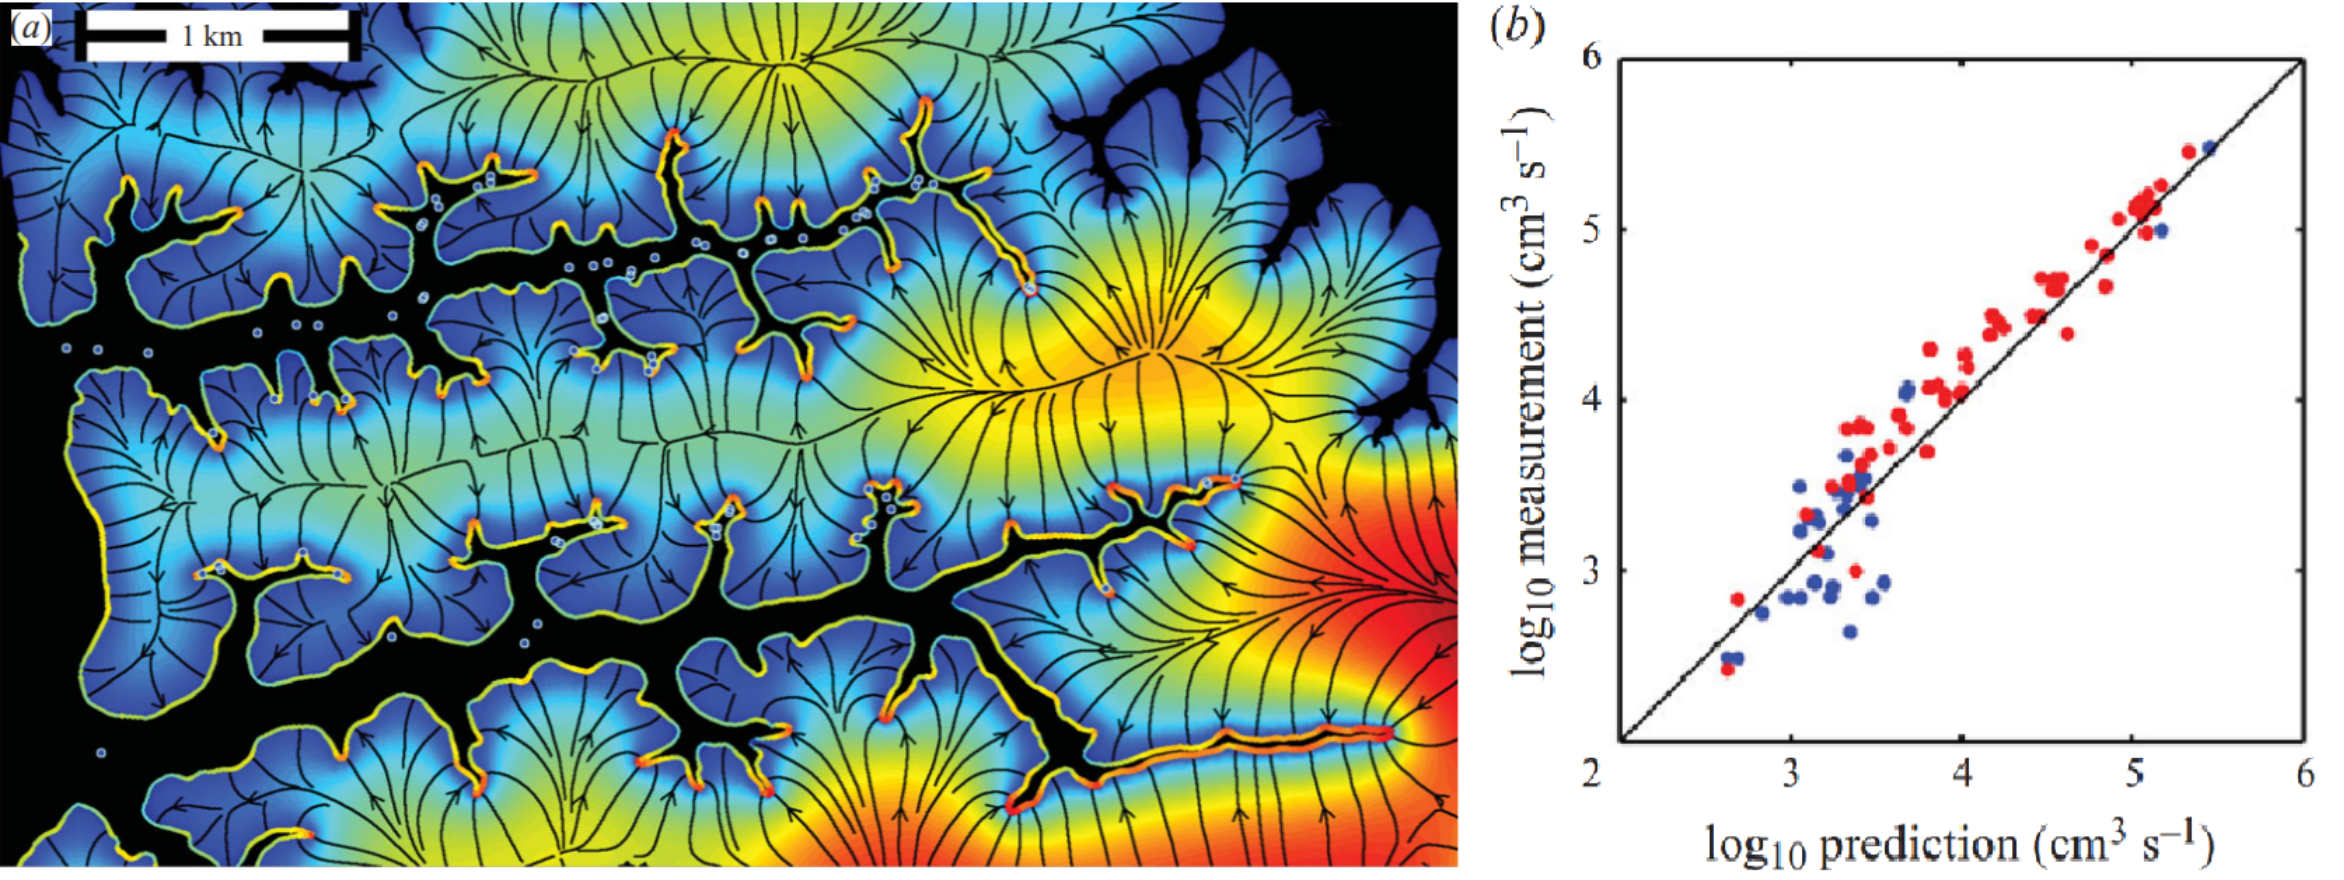
\includegraphics[width=\textwidth]{figs/potencjal_floryda_przewidywania.png}
      \caption{Zwierciadło wód gruntowych i związany z nim przepływ wód gruntowych w sieci na Florydzie \cite{petroff2011geometry}. (a)~Wielkość obliczonego pola Poissona (b)~Porównanie przewidywanego zrzutu z pomiarami w 30 punktach sieci wykonanych w styczniu 2009 (punkty niebieskie) i 52 punktach w kwietniu 2009 (punkty czerwone). Czarna linia oznacza równość. To porównanie jest bezpośrednie i nie wymaga regulowanych parametrów.}
      \label{potencjal_floryda}
    \end{figure}



  \chapter{Rozwiązywanie równania Laplace'a}\label{chapter:solving}
    
    Usunięcie UW-niestabilności interfejsu poprzez przybliżenie cienkiego palca ma swoją cenę. Po pierwsze, pole na wierzchołku staje się pojedyncze, a dokładniej gradient pola rozchodzi się jak $r^{-1/2}$ w pobliżu wierzchołka. We współrzędnych biegunowych (gdzie kierunek stycznej do palca na wierzchołku ustawia $\theta = 0$ -- patrz rys. \ref{grid_pot}) pole w pobliżu wierzchołka można rozszerzyć \cite{derrida1992needle , petroff2013bifurcation}:
    
    \begin{equation}\label{phi_polar}
      \phi(r,\theta)=a_1r^{1/2}\cos\frac{\theta}{2}+a_2r \sin \theta+a_3 r^{3/2} \cos\frac{3\theta}{2}+\mathcal{O}\left(r^2\right) \,,
    \end{equation}

    gdzie współczynniki $a_i$ zależą od warunków brzegowych daleko od czubka palca. Równ. \eqref{phi_polar} obowiązuje również w przypadku pól Poissona, ponieważ w sąsiedztwie wierzchołka wkład strumienia z członu źródłowego jest pomijalny w porównaniu do strumienia z obszarów oddalonych od wierzchołka. Dla każdego z wiodących współczynników $a_i$ w równaniu \eqref{phi_polar} możemy znaleźć interpretację fizyczną (rys. \ref{grid_pot}).

    \begin{figure}[H]
      \centering
      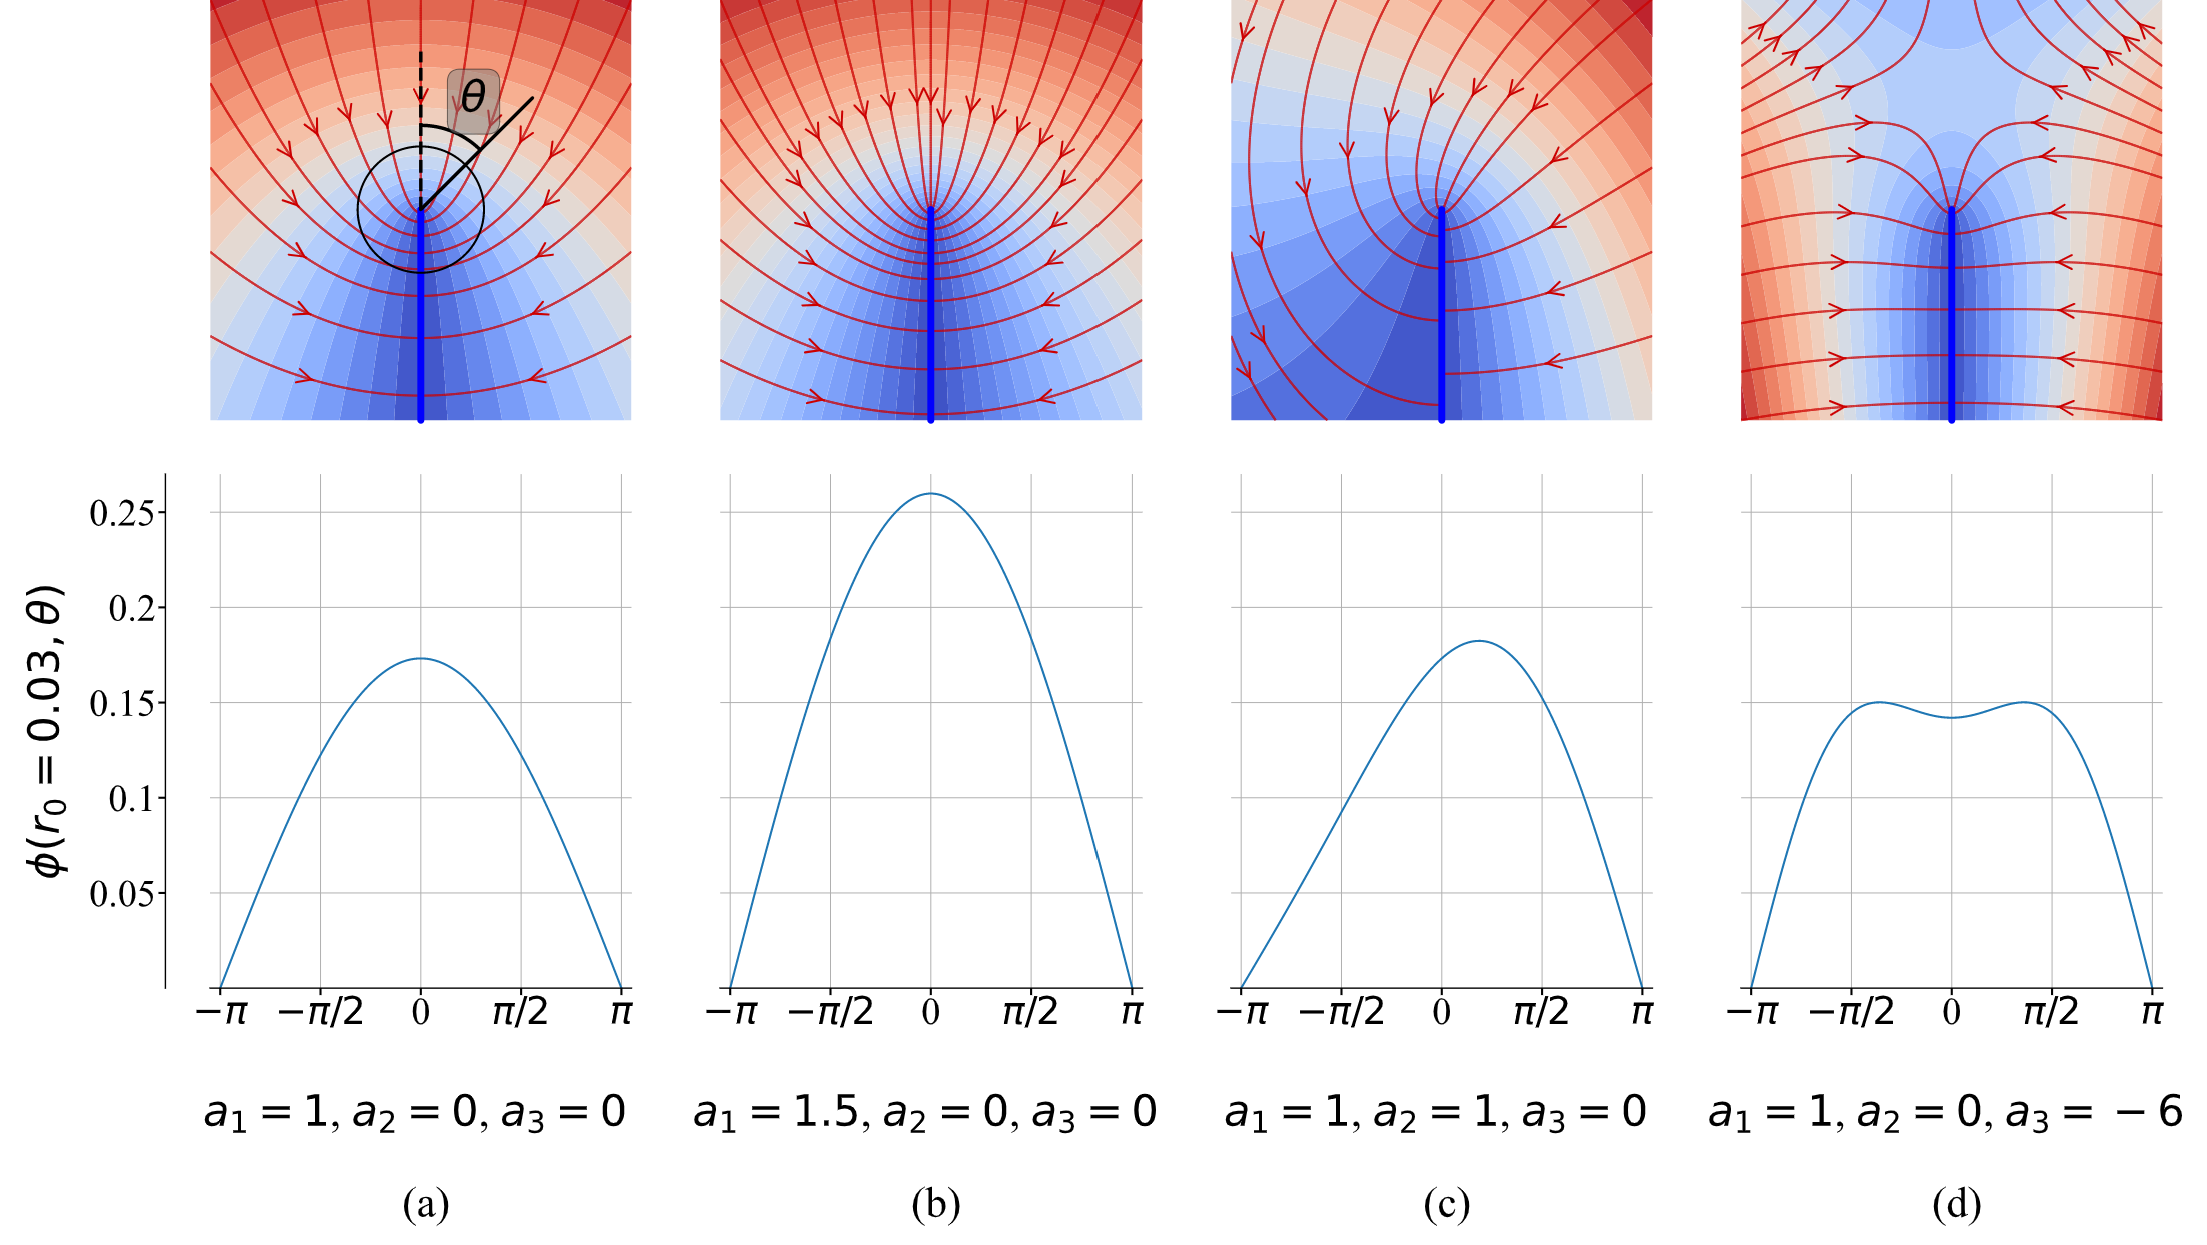
\includegraphics[width=0.93\textwidth]{figs/grid_potential_python.png}
      \vspace{0pt}
      \caption {Pole wokół opuszki palca (niebieska linia pośrodku) dla różnych $a_1, a_2, a_3$ (po Ref.~\cite{petroff2013bifurcation}). W górnym rzędzie kolory od czerwonego do niebieskiego są powiązane z wielkością pola, a czerwone strzałki podążają za liniami pola. Dolny rząd przedstawia profile pola wzdłuż małego okręgu wokół wierzchołka (czarne kółko w górnym rzędzie).}
      \label{grid_pot}
    \end{figure}

    Po pierwsze, współczynnik $a_1$ jest powiązany z całkowitym strumieniem na małym okręgu o promieniu $r_0$ wokół końcówki (rys.~\ref{grid_pot}a, b):
    
    \begin{equation}\label{circle}
      J|_{r_0} = \oint_{r_0} (-\kappa \nabla \phi) \cdot \hat{n} \ \textrm{d}l = 2 \kappa a_1 r_0^{1/2} + \mathcal{O}\left(r_0^{3/2}\right) \,.
    \end{equation}

    Współczynnik $a_2$ jest powiązany z asymetrią pola wokół wierzchołka (Rys.~\ref{grid_pot}c). Przy dodatnim $a_2$ strumień pola jest większy po prawej stronie wierzchołka, a przy ujemnym $a_2$ — po lewej stronie. Palec rośnie jednak w kierunku największego strumienia i w efekcie rośnie w taki sposób, że $a_2$ zawsze znika (zasada lokalnej symetrii \cite{cohen2015path}).
    
    Wreszcie $a_3$ jest połączona z drugą pochodną pola. Jeśli ponownie skupimy się na małym okręgu o promieniu $r_0$ wokół końcówki i zbadamy pole jako funkcję kąta $\theta$, zauważymy, że przy ustalonych $a_1>0$ i $a_2=a_3=0$ pole ma pojedyncze maksimum przy $\theta = 0$ (rys. \ref{grid_pot}a, b). Im mniejszy współczynnik $a_3$, tym bardziej płaskie maksimum pola wokół końcówki. W końcu, gdy druga pochodna $\phi$ znika, co odpowiada ujemnej wartości $a_3/a_1$:
    
    \begin{equation}\label{a3a1}
      \frac{\partial^2 \phi}{\partial \theta^2}\big|_{\theta=0, r=r_0} = 0 \implies a_3/a_1 = -\frac{1}{9 r_0} \,, 
    \end{equation}
    
    to pojedyncze maksimum przekształca się w dwa maksima w $\pm \theta_0$ (rys. \ref{grid_pot}d). Zauważ, że wartość progowa $a_3/a_1$ zależy od odległości $r_0$ od końcówki, przy której analizowane jest pole. Dla nieskończenie małych $r_0$ profil pola jest zawsze symetryczny z jednym maksimum przy $\theta=0$.

    Aby otrzymać współczynniki $a_i$, możemy po prostu rozwiązać odpowiednie równanie dla pola (Laplace'a lub Poissona) metodą elementów skończonych, a następnie korzystając z postaci całkowej współczynników:
    
    \begin{equation}
      \label{a1}
      a_1 = \frac{1}{\pi r_0^{1/2}}\int^{\pi}_{-\pi} \phi(r_0,\theta)\cos\frac{\theta}{2}\textrm{d}\theta \,,
    \end{equation} 
    
    \begin{equation}
      \label{a2}
      a_2 = \frac{1}{\pi r_0}\int^{\pi}_{-\pi} \phi(r_0,\theta)\sin\theta \textrm{d}\theta \,,
    \end{equation}
    
    \begin{equation}
      \label{a3}
      a_3 = \frac{1}{\pi r_0^{3/2}}\int^{\pi}_{-\pi} \phi(r_0,\theta)\cos\frac{3\theta}{2}\textrm{d}\theta
    \end{equation}	
    
    obliczyć je. Przeprowadzamy ją w programie RiverSim który był inspirowany rozwiązaniem w FreeFEM++\cite{hecht2012new} początkowo stworzonych przez grupę Daniela Rothmana w MIT \cite{petroff2011geometry, petroff2013bifurcation, cohen2015path} i dalej rozwijanych w grupie Piotra Szymczaka \cite{morawiecki2016problem, zukowski2019zwiazek}.



  \chapter{Ewolucja naprzód}
    
    \section{Reguły wzrostu}

      Możemy teraz przejść do opisu reguł wzrostu systemu wyposażonego we współczynniki $a_i$. W najogólniejszym przypadku prędkość wzrostu może być dowolną funkcją pola ($v = f(\phi)$), ale w klasycznym wzroście Laplace'a jest proporcjonalna do gradientu pola -- $f(\phi) = \alpha |\nabla \phi|$, gdzie $\alpha$ jest stałą proporcjonalności. Jednak, prawo potęgowe zostały odnotowane w wielu różnych systemach fizycznych, np. przebicie dielektryczne \cite{niemeyer1984fractal} i -- po tych pracach -- założymy tutaj, że prędkość końcówki jest proporcjonalna do strumienia wchodzącego w nią pola ($J$) do potęgi $\eta$. Przypominając równanie \eqref{circle} mamy \cite{carleson2002laplacian, selander1999two}:
      
      \begin{equation}\label{velocity}
        v = \alpha a_1^\eta \,.
      \end{equation}
      
      Problem wolnej granicy Saffmana i Taylora ma wewnętrzną niestabilność, która dzieli jeden palec na dwie gałęzie potomne w zależności od szerokości palca i prędkości \cite{lajeunesse2000tip}. I odwrotnie, palce w modelu cienkich palców nie rozdzielają się naturalnie. Dlatego, aby tworzyć rozgałęzione sieci, musimy wprowadzić regułę podziału. Ilekroć taka reguła podziału jest spełniona, tworzymy dwie gałęzie potomne w $\theta = \pm 36^\circ$ (mierzone w układzie współrzędnych wokół wierzchołka, jak poprzednio) -- jak pokazano w Odn. \cite{hastings2001growth, carleson2002laplacian, gubiec2008fingered, devauchelle2012ramification} kąt otwarcia bifurkacji w modelu z cienkimi palcami wynosi 72$^\circ$. W literaturze dotyczącej modelu cienkiego palca stosuje się dwa różne deterministyczne kryteria podziału -- kryterium prędkości i kryterium kształtu pola.

      Pierwsza opiera się na obserwacji, że długość fali niestabilności $\lambda_c$ maleje wraz ze wzrostem prędkości propagacji przedniej \cite{pecelerowicz2016stabilizing}. Gdy palec w pewnym momencie przyspiesza, $\lambda_c$ staje się mniejsza niż jego szerokość i ulega destabilizacji (rys. \ref{wavelength}). Takie kryterium może być wprost zaimplementowane w modelu cienkiego palca jako próg $a_1$: $a_1 > a_1^c$.
      
      \begin{figure}[H]
        \centering
        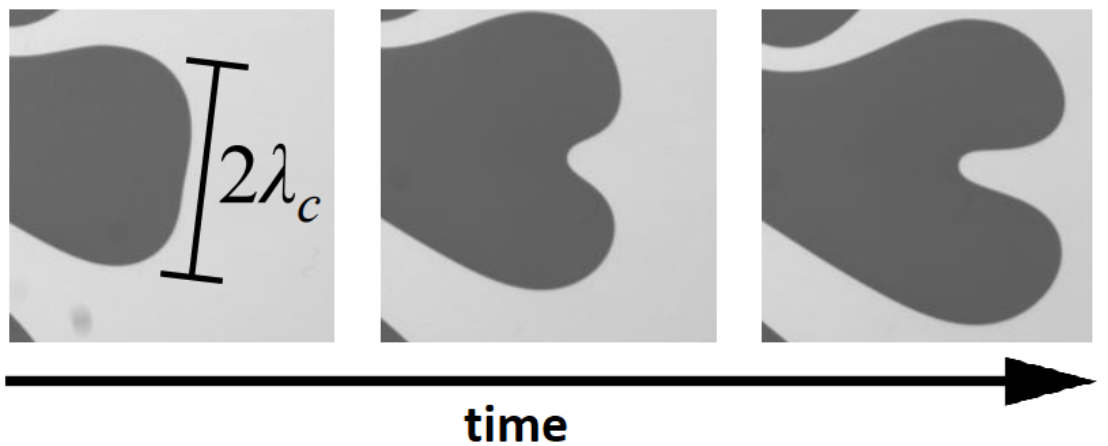
\includegraphics[width=0.475\textwidth]{figs/wavelength.png}
        \vspace{-10pt}
        \caption{Kryterium prędkości bifurkacji: $v > v_{c}$. Migawki przesuwających się palców w eksperymencie lepkiego palcowania \cite{bischofberger2015island}.}
        \label{wavelength}
      \end{figure}

      Drugie kryterium jest związane z ekstremami strumienia (w funkcji kąta biegunowego) \cite{petroff2013bifurcation, kaandorp2001algorithmic_Chapter4.4}, a więc ze współczynnikiem $a_3$. Gdy dla danego promienia $r_0$ strumień pola ma wysokie pojedyncze maksimum, palec rośnie w kierunku tego maksimum. Jeśli jednak strumień pola z boków wierzchołka staje się porównywalny do tego z przodu, a nawet w końcu staje się większy (co odpowiada pojawieniu się dwóch maksimów przy $\pm \theta_0$), palec próbuje rosnąć w dwóch kierunkach jednocześnie, co skutkuje bifurkacją. Mówiąc dokładniej, mówimy, że palec dzieli się, gdy $a_3/a_1$ jest mniejsze niż jakaś wartość krytyczna.

      \begin{figure}[H]
        \centering
        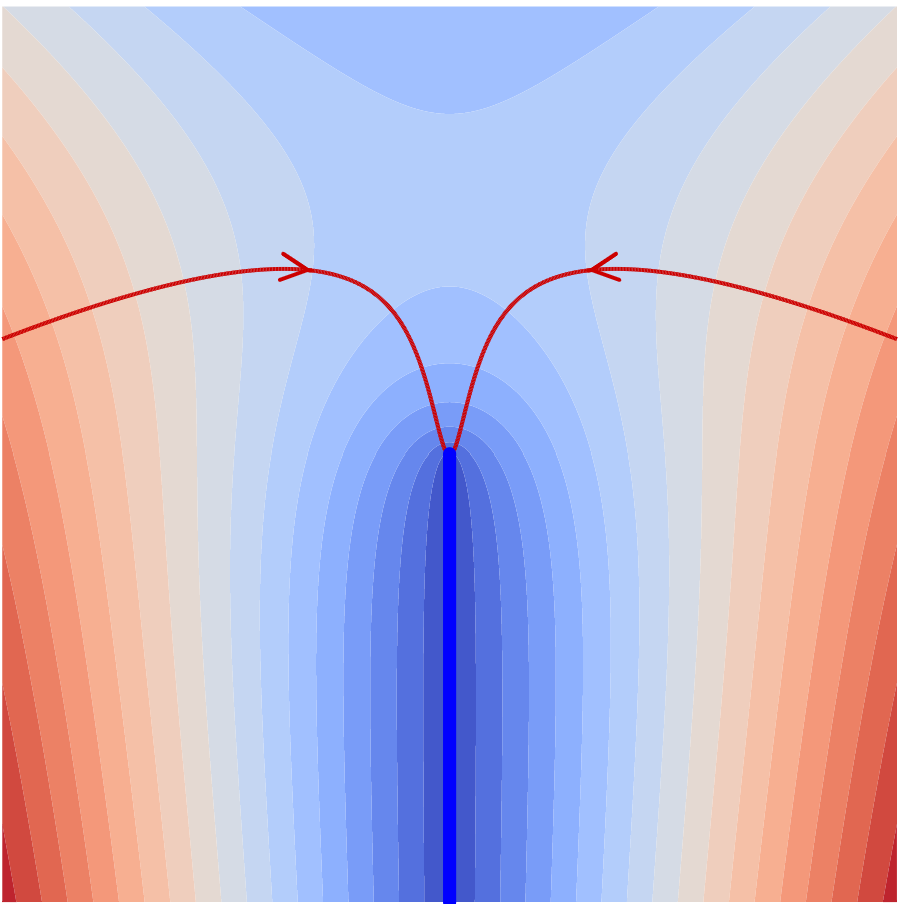
\includegraphics[width=0.4\textwidth]{figs/bifurcation_rule_a3.png}
        \caption{Kryterium kształtu pola bifurkacji: $a_3/a_1 < \textrm{wartość krytyczna} $. Na działce linie pola wchodzące w okrąg wokół czubka z dwóch stron.} 
        \label{bif_rule_a3}
      \end{figure}


    \section{Algorytm ewolucji do przodu}

      Biorąc pod uwagę zasady rozwoju, możemy symulować rozwój sieci. Poza najprostszymi przypadkami rozwiązań jedno- i dwupalcowych \cite{gubiec2008fingered} trzeba sięgnąć do metod numerycznych, aby znaleźć ewoluującą geometrię sieci. Najpierw sprawiamy, że równania są bezwymiarowe, przeskalowując współrzędne w następujący sposób: $x' = \frac{x}{w}$ (przy czym $2w$ to szerokość układu), $t' = \alpha w^{\ frac{3}{2}\eta-1} (\frac{\mu P}{\kappa})^{\eta} t$ (z $\alpha$ zdefiniowanym w równaniu~\ref{velocity}), oraz pole: $\phi' = \frac{\kappa}{w^2 \mu P}\phi$. To prowadzi do:
      
      \begin{gather}
        \label{rescaled_poisson} \Delta^\prime \phi^\prime = -1 \\ 
        \label{rescaled_vel} v' = (a'_1)^\eta
      \end{gather}

      Przeskalowanie przypadku Laplace'a ($P=0$) jest nieco inne. Tutaj system jest zwykle zasilany przez strumień pola wychodzący z granicy ($J_0$), więc $P$ w przeskalowaniu jest zastępowane przez $J_0 / w$. Teraz $t' = \alpha w^{\frac{1}{2}\eta-1} (\frac{\mu J_0}{\kappa})^{\eta} t$, a pole: $ \phi' = \frac{\kappa}{w \mu J_0}\phi$ i równ. \eqref{rescaled_poisson} zostaje zastąpiony przez:
      
      \begin{equation}
        \Delta^\prime \phi^\prime = 0 \,.
      \end{equation}

      Przeskalowanie $\phi^\prime$ i $x^\prime$ wpływa również na współczynniki $a_i$ -- ich jednostki są teraz wyrażone w ujemnych potęgach $w$. Dla wygody upuszczamy liczby pierwsze dla przypadków bezwymiarowych w pozostałej części artykułu.

      Nasz algorytm wzrostu składa się z następujących elementów. Na początku określamy granice domeny oraz wyjściową geometrię sieci. Następnie w każdym kroku czasowym rozwiązujemy równanie Laplace'a ($\Delta \phi = 0$) lub Poissona ($\Delta \phi = -1$) dla pola metodą elementów skończonych i obliczamy $a_1 , a_2, a_3$ współczynniki dla każdej końcówki. Na podstawie obliczonej wartości $a_1$ i równania. \eqref{rescaled_vel} otrzymujemy przemieszczenie każdego wierzchołka w czasie $\textrm{d}t$: $\textrm{d}s = v \textrm{d}t = a_1^\eta \textrm{d}t$ . Trajektorię palca można uzyskać wykorzystując fakt, że wzrost przebiega wzdłuż linii opływowej wchodzącej w końcówkę (jest tylko jedna taka linia opływowa). Dla małych przemieszczeń $\textrm{d}s$ otrzymujemy ($\beta = \frac{a_1}{a_2}$):

      \begin{figure}[h]
        \centering
        \begin{minipage}{0.25\textwidth}
          \centering
          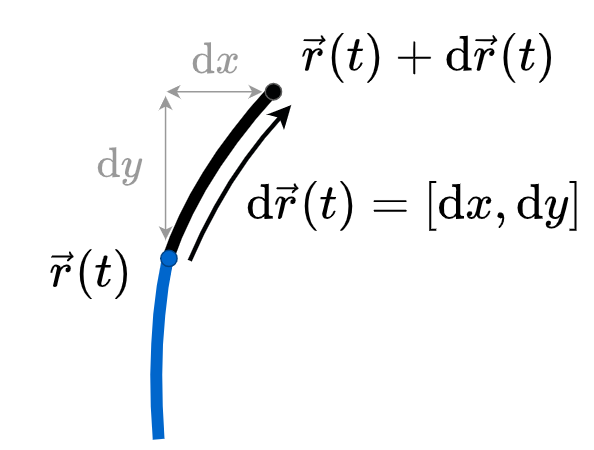
\includegraphics[width=\textwidth, trim={0 0 285 0},clip]{figs/growth.png}
        \end{minipage}
        \hspace{-40pt}
        \begin{minipage}{0.6\textwidth}
          \begin{align}
            \label{x_growth}
            & \textrm{d}x(\textrm{d}y)=2\sqrt{\frac{\textrm{d}y(\textrm{d}s)^3}{\beta^2}+\frac{\textrm{d}y(\textrm{d}s)^4}{\beta^4}}\\
            \label{y_growth}
            & \textrm{d}y(\textrm{d}s)=\frac{\beta^2}{9}\left[\left(\frac{27 \textrm{d}s}{2 \beta ^2}+1\right)^{2/3} - 1 \right]
          \end{align}
        \end{minipage}
        \vspace{0pt}
      \end{figure}

      Aby uniknąć problemów ze znacznymi różnicami w krokach przestrzennych ze zmiennymi gradientami pola podczas ewolucji sieci, dostosowujemy wartość $\textrm{d}t$ w każdym kroku czasowym, aby zachować $\textrm{d}s$ najszybsza stała gałęzi.

  \section*{Acknowledgements}
    Dziękuję Piotrowi Morawieckiemu za pomoc w zrozumieniu jego kodu. Solver numeryczny został oparty na pakiecie opracowanym przez grupę Daniela Rothmana z MIT. Szczególnie dziękujemy Olivierowi Devauchelle z Institut de Physique du Globe w Paryżu i Hansj\"{o}rg Seyboldowi z ETH Zurich za udostępnienie tego kodu i wszelką pomoc.

\end{document}